\chapter{Introduction}
% scatteringPerhaps the best way to introduce the current state of particle
% physics is to start with a historical\footnote{by no means I
%   pretend to have a rigorous historical approach but rather summarize
%   the scientific triumphs that shaped what particle physics is today}
% approach. The beginning of modern particle physics starts in 1897 with the
% discovery of electron by J. J. Thomson while he was studying cathode
% rays. Thompson determined that the charge-to-mass ratio was extremely
% large and therefore a new particle with negative charge and extremely
% light was necessary to explain the observations. Later came, continuing the
% path of what is sometimes called classical particle physics,
% Rutherford's famous scattering experiment, which by recording the
% angles of the outgoing $\alpha-$particles scattered off a gold foil,
% reached the astonishing conclusion that the majority of the charge and
% mass of the atom is contained in a small region in space, the
% nucleus. The nucleus of the lightest element -- hydrogen, which has an
% electron orbiting the nucleus -- is what we know as the
% proton. Spectacular agreement between the theoretical predictions and
% the experimental measurements of the spectrum of hydrogen gave
% credibility to atomic model. Thus, it is was proposed that the rest of
% the elements, which are heavier, will have just more protons in the
% nucleus and the corresponding number of electron orbiting it. This
% picture was immediately proved wrong since the mass of the next
% element, helium, was measure to approximately weigh 4 times as much as
% hydrogen. Although wrong, this model correctly predicted the number of
% electrons. Therefore the somewhat obvious solution was to set the number of protons to match that of electron -- so that the
% net charge of the atom is zero -- and introduce a neutral particle
% with the same mass as the proton, the neutron. The neutron was
% discovered by Chadwick in 1932 and thus completed the atomic
% model. During the same period of time, i.e. 1900-1924, another
% scientific revolution was developing, this revolution will paved the
% road to the principles of quantum mechanics and proposed a new
% fundamentally different particle, the photon. The photon discovery
% started in 1900, when Planck introduced it in order to explain the
% observed blackbody spectrum -- the spectrum of the
% electromagnetic radiation emitted by a hot object. In order to
% overcome the difficulties of statistical mechanics in explaining the
% blackbody spectrum, Planck had to introduce the radical notion that electromagnetic radiation was \textit{quantized}, this is to say, that
% it only comes in small energy ``packages'' (quanta), these quanta
% carry an energy proportional to the frequency of the electromagnetic
% radiation ($E = h\nu$). Although this quantization of the energy did
% solve the blackbody spectrum problem, Planck did not believe that the
% quantization was part of reality. By 1905, perhaps the most well know
% physicist, Albert Einstein proposed that the quantization was indeed
% inherent to the electromagnetic field. He used this idea to explain
% the \textit{photoelectric effect}. When the surface of a metal is hit
% by electromagnetic radiation, electrons are release with a particular
% energy. Einstein argued that a quantum of light transferred all its
% energy ($h\nu$) to an electron, then the excited electron upon
% traveling out of the material will loose a determined amount of energy
% (the work function, $w$); therefore the energy of the outgoing electron is
% $E\leq h\nu - w$. Despite of the experimental success of the
% photoelectric effect theory, measured by Millikan in 1916, the
% community was not willing to accept the quantization idea as a
% fundamental part of nature. Finally, in 1923 A. Compton
Particle physics is perhaps facing one of the biggest crossroads since
the discovery of the electron in 1897. The subject evolved from having
just one particle to have a catalog of particles and their possible
interactions, and even explain the origin of the particles
masses. This knowledge is encoded in what we know today as the
Standard Model (SM) of particle physics, the most precise and perhaps
the most successful theory that mankind has ever had. The SM is a
quantum filed theory that sets the
rules by which the particles that we have observed interact with each
other. These interactions compose three of the four fundamental force
we know: the strong, weak, and electromagnetic interactions, leaving
gravity aside. Most of the predictions since its formulation (mostly
during the 1960s) have been experimentally observed: we have measured the W and Z
bosons, the top quark, and recent the discovery of the last piece of
the puzzle by the ATLAS and CMS
collaborations~\cite{CMSHIGGS,ATLASHIGGS}, the Higgs boson. However, despite the success and completeness of
the SM, we are now faced with fundamental questions, both experimentally and theoretically motivated, 
that are unfortunately not answered:

\begin{itemize}
\item Why is Higgs boson mass at the weak scale since its mass is
  sensitive to a high energy scale through radiative corrections (fine
  tuning)?
\item Is there a unification of the gauge couplings at the Planck scale?
\item What is the nature of \textit{dark matter}, whose existence
  has only been inferred by astrophysical measurements?
\item What is the nature of the matter/anti-matter asymmetry observed
  in the universe?
\item  What is the nature of \textit{dark energy}, whose existence provides an
  explanation for the expansion of the universe?
\item Is there a quantum theory of gravity?
\end{itemize} 

This thesis is more concerned with the first three bullets, which can
actually be answered with a single theory: \textit{supersymmetry}, a
quantum field theory that relates fermions, and bosons~\cite{susy1,susy2,susy3,susy4,susy5,susy6,susy7}, which tackles
these questions by adding a dark matter candidate to the
particle spectrum, unifying the gauge couplings at the Planck scale,
and alleviating the fine tuning of the Higgs mass.

Although supersymmetry is a very compelling theoretical framework, it is not needed for having
a suitable dark matter candidate. In fact, in order to match
the observed dark matter relic density, there are just two
conditions that need to be satisfied. These are the strength of the interaction of the dark matter (DM)
candidate -- here it is assumed that the DM candidate is a fundamental
particle -- with the SM particles is at the level of the weak interaction,
and the mass of the DM candidate is about 100\GeV. This realization is
called the \textit{weakly interacting massive particle (wimp)
  miracle}. This led to the idea that DM candidates can be
produced at particle colliders by just inverting the direction of
interaction, i.e. two SM particles annihilating into two DM
candidates. Unfortunately, this event topology will leave no trace on the particle
detectors due to the weakly interacting nature of the DM candidate,
and therefore another particle must be produced in the event; the latter is
easily resolved by the production of additional particles via
initial-state radiation (ISR) off the incoming SM
particles. All of the above led to collider searches in events with one highly-energetic jet
or photon and substantial momentum imbalance. These searches became known as \textit{monojet}~\cite{Aad:2011xw,Chatrchyan:2012me} and
\textit{monophoton}~\cite{Khachatryan:2014rwa,Aad:2014tda},
respectively.

Another line of thought, more experimentally driven one might say, is
the fact that there has to be new phenomena, since the SM falls short
on explaining some of the current experimental observations. This realization gives
ground to what is called \textit{model-independent} searches, in which
the events are selected based on interested topologies rather than a
particular theoretical models. Examples of such data analyses are dijet and
diphoton resonance searches at relatively high masses. Another way to
probe new physics is to search for anomalous production of Higgs
bosons, where new phenomena could enhance the SM Higgs production or
decay rates. These searches have recently been enabled by the
measurements of the Higgs boson properties.

The broad experimental programs established by the ATLAS and CMS
collaborations rely on the good performance of the particle detectors,
reconstruction algorithms, as well as the large datasets provided by
the large Hadron Collider (LHC). The High-Luminosity upgrade of the
LHC will significantly boost the sensitivity to rare processes but at
the cost of increasing the pileup interactions to about 200. This high
pileup environment will deteriorate particle reconstruction and
identification due to the large occupancy in the detector. One
solution to alleviate this detrimental effect is to have a
calorimetric device capable of delivering a time stamp for particle
detection with a resolution of about 30 ps (approximately 1 cm in the
z-axis). Detector research and  development (R\&D) is crucial in order
to make precision timing calorimetry a reality that could enhance the
potential discovery and characterization of new physics. 


This thesis is organized in five parts: the first part gives a brief
introduction to the main theoretical and phenomenological
considerations covered by the experimental searches in the following
parts; the second part provides an introduction to the Large Hadron
Collider and the Compact Muon Solenoid Experiment where the searches
presented in this thesis are carried out; the third part covers in
detail two searches for beyond the SM (BSM) physics with \textit{razor variables} using data collected by
the CMS experiment at a center-of-mass energy of 8\TeV and 13\TeV; the
fourth part presents the research and development on precision timing
calorimetry that we carried out at Fermilab and CERN; the fifth part -- the appendices
-- presents another search for new resonances in high-mass diphotons using 13\TeV data collected by the CMS experiment as well
as a reinterpretation of the excess observed by CMS in events with SM
Higgs produced in association with jets at 8\TeV.


\chapter{The Standard Model in a Nutshell}
\section{The Standard Model of Particle Physics}
The Standard Model (SM) of particle physics is a renormalizable
quantum field theory based on symmetries and the gauge principle~\cite{HOOF,WeinbergLeptons}. The
SM explains the electromagnetic, weak, and strong interactions, as
well as having a complete catalog of all subatomic particles
known. The interactions between the fermions (spin 1/2 particles) is
realized by the exchange of force carriers (spin-1 particle).

The SM is represented by the symmetry group $\mathrm{SU(3)_{C}} \times
\mathrm{SU(2)_{L}} \times \mathrm{U(1)_{Y}}$, where each of the
fundamental forces, represented by gauge fields, corresponds to one of
symmetry groups. This is better understood by the following
diagrammatic representation:

\begin{center}
\begin{tabular}{ c c c c c }
  $\mathrm{SU(3)_{C}}$ & $\times$ & $\mathrm{SU(2)_{L}}$ & $\times$ & $\mathrm{U(1)_{Y}}$\\
  $\downarrow$ &  & $\downarrow$ & & $\downarrow$\\
  $G^{\alpha}_{\mu}$ &  & $W^{a}_{\mu}$& &$B_{\mu}$ \\
  $\alpha = 1,\cdots,8$ & & $a = 1,2,3$ & & \\
\end{tabular}
\end{center}

Where $G^{\alpha}_{\mu}$ represents the eight boson, the gluons, that take part in
the strong interaction and are associated with the
$\mathrm{SU(3)_{C}}$ term;  $W^{a}_{\mu}$ represents the three bosons
that take part in the weak interaction and are associated with the
$\mathrm{SU(2)_{L}}$; while $B_{\mu}$ represents the boson associated
with the hyper-charge $\mathrm{U(1)_{Y}}$ term. The latter four bosons
mix to form the most commonly known $W^{\pm}$ and $Z$ bosons of the
weak interaction, and the photon ($\gamma$) of the electromagnetic
interaction.

The particles that make up matter are represented by fermion fields in
the form of left- and right-handed Weyl spinors. These fermions are
divided into two categories, quarks (u, d, c, s, t, and b), and
leptons (e, $\mu$, $\tau$, $\nu_{e}$, $\nu_{\mu}$, and
$\nu_{\tau}$). Quarks are the only fermions that experience the strong
interaction. Both, quarks and fermions, are further categorized into
three generations of matter -- where e, u, and d are in the first
generation and $\tau$, t and b are in the third generation --, with
particles masses increasing in the same order as the
generations. Figure~\ref{fig:SMcartoon} shows the whole catalog of
particles and interactions in the standard model, including their
categorization, and the Higgs boson which will be discussed in the
following section.
\begin{figure}
 \centering
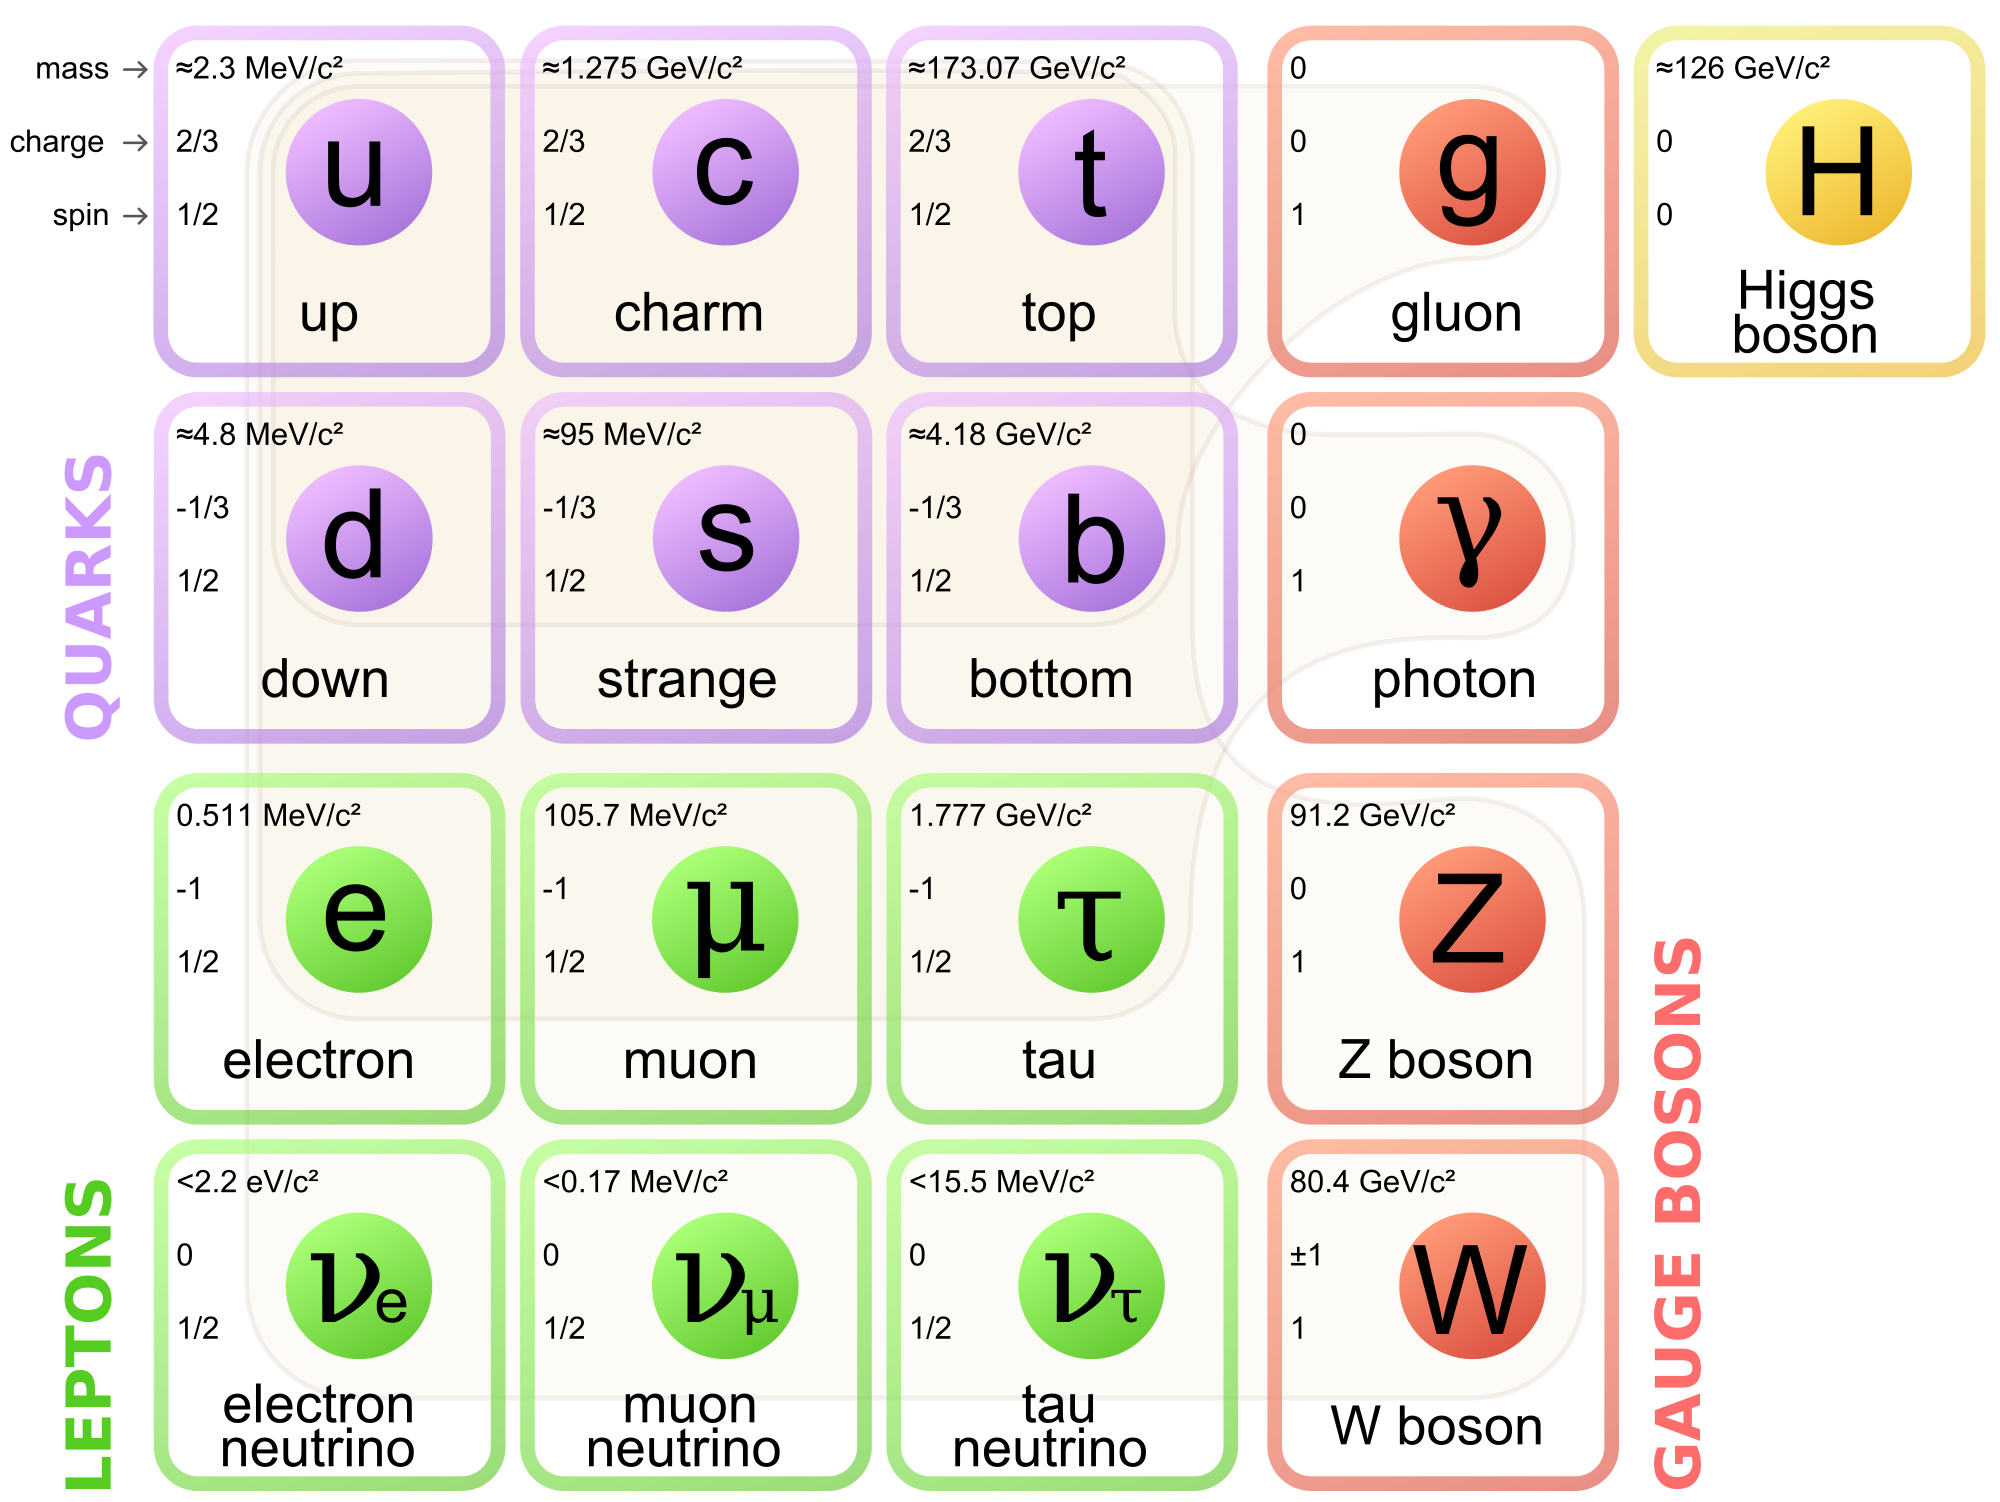
\includegraphics[width=0.9\textwidth]{IntroFigures/TheSM.png}
 \caption{The catalog of particles in the standard model.\label{fig:SMcartoon}}
\end{figure}

The dynamics and kinematics of the SM are controlled by the
Lagrangian density, which in conjunction with the particle content and
force carriers completes the theory. The Lagrangian density is
presented below in compact formulation:
\begin{equation}
 \begin{aligned}
        \mathcal{L}_{\mathrm{SM}}& = -\frac{1}{4}B_{\mu\nu}B^{\mu\nu}
        -\frac{1}{4}W^{a}_{\mu\nu}W^{\mu\nu}_{a} - \frac{1}{4}G^{\alpha}_{\mu\nu}G^{\mu\nu}_{\alpha} 
        \qquad \text{gauge terms}\\
        &+\bar{\ell}_{\mathrm{L}}\tilde{\sigma}^{\mu}iD_{\mu}\ell_{\mathrm{L}}
        +\bar{e}_{\mathrm{R}}\sigma^{\mu}iD_{\mu}e_{\mathrm{L}} +
        \bar{\nu}_{\mathrm{R}}\sigma^{\mu}iD_{\mu}\nu_{\mathrm{L}} \qquad \text{lepton kinetic terms}\\
        &+\bar{q}_{\mathrm{L}}\tilde{\sigma}^{\mu}iD_{\mu}q_{\mathrm{L}}
        +\bar{u}_{\mathrm{R}}\sigma^{\mu}iD_{\mu}u_{\mathrm{L}} +
        \bar{d}_{\mathrm{R}}\sigma^{\mu}iD_{\mu}d_{\mathrm{L}} + \qquad \text{quark kinetic terms}\\
        &+\mathcal{L}_{\mathrm{Higgs}} +
        \mathcal{L}_{\mathrm{Yukawa}}\qquad \text{Higgs and Yukawa terms}
       \end{aligned}
\label{eq:theSMlagrangian}
\end{equation}

Where $\ell_{\mathrm{L}}=\begin{pmatrix}e_{\mathrm{L}}\\
  \nu_{\mathrm{L}}\end{pmatrix}$ is the lepton $\mathrm{SU(2)_{L}}$
doublet, $q_{\mathrm{L}}=\begin{pmatrix}u_{\mathrm{L}}\\
  d_{\mathrm{L}}\end{pmatrix}$ is the quark $\mathrm{SU(2)_{L}}$
doublet, $D_{\mu}$ is the corresponding covariant derivative, and
 $\sigma_{mu}$ is the identity and the Pauli matrices ($\sigma_{\mu} = {1,\sigma^{i}}$).
The $\mathcal{L}_{\mathrm{Higgs}}$ and $\mathcal{L}_{\mathrm{Yukawa}}$
are presented in sections~\ref{higgs} and~\ref{yukawa}, respectively.
Table~\ref{tab:SMGroup} presents the matter field representation in
the SM gauge group.

\begin{table}[htb]
\centering
\large
\begin{tabular}{cccc}
  \hline
  \hline
  field &  $\mathrm{SU(3)_{C}}$ &  $\mathrm{SU(2)_{L}}$ & $\mathrm{U(1)_{Y}}$\\
  \hline                                                        
  $q_{L}$ & $\mathbf{3}$ &  $\mathbf{2}$ & 1/6\\
  $\ell_{L}$ & $\mathbf{1}$ &  $\mathbf{2}$ & -1/2\\
  $u_{R}$ & $\mathbf{\bar{3}}$ &  $\mathbf{1}$ &-2/3\\
  $d_{R}$ & $\mathbf{\bar{3}}$ &  $\mathbf{1}$ &1/3\\
  $e_{R}$ & $\mathbf{1}$ &  $\mathbf{1}$ & 1\\
  $h$ & $\mathbf{1}$ &  $\mathbf{1}$ & 1/2\\
  \hline
  \hline
\end{tabular}
  \caption{\label{tab:SMGroup} Group representation of the matter
    fields in the SM.}
\end{table}
\section{The Higgs Boson and Electroweak Symmetry
  Breaking}\label{higgs}
Gauge theories prohibit -- in order to maintain the local symmetries --  explicit mass terms for the gauge bosons in the SM,
therefore all gauge bosons are massless. Since some of gauge boson in
the SM are massive ($W^{\pm}$,$Z$) there should be a mechanism by
which gauge boson acquire mass. The gauge boson masses in the SM are
realized by the \textit{spontaneous symmetry breaking} of the
$\mathrm{SU(2)_{L}}\times U(1)_{\mathrm{Y}}$ symmetry which induced by the nature of
the Higgs potential~\cite{Englert,HIGGS1,HiGGS2,Guralnik,HIGGS3,Kibble}. The best way to understand this mechanism (the
Higgs mechanism) is to closely look at the Lagrangian density:

\begin{equation}
\label{eq:higgsPotential}
\mathcal{L}_{\mathrm{Higgs}} =
(D^{\mu}\mathbf{\Phi})^{\dagger}(D^{\mu}\mathbf{\Phi}) +
V(\mathrm{\Phi});\hspace{1cm} V(\mathrm{\Phi}) = -\mu^{2}\Phi^{\dagger}\Phi +\lambda(\Phi^{\dagger}\Phi)^{2},
\end{equation}
where $D^{\mu}$ is the covariant derivative; $\Phi$ is a spin-0
complex field, and a $\mathrm{SU(2)_{L}}$ doublet with weak
hyper-charge $\mathrm{Y} = 1/2$. The field is more easily represented
as a $\mathrm{SU(2)_{L}}$ doublet in the following fashion:
\begin{equation}
\label{eq:higgdoublet}
\Phi = \begin{pmatrix} \phi^{+}\\
  \phi^{0}\end{pmatrix}.
\end{equation}

When $\mu^{2} > 0$ the potential ($V(\Phi)$) has the commonly known
``Mexican hat'' shape, shown in Figure~\ref{fig:MexHat}, with a minimum which does not preserve the
original $\mathrm{SU(2)_{L}}\times U(1)_{\mathrm{Y}}$
symmetry. Therefore the scalar field acquires a non-zero
\textit{vacuum expectation value (vev)}:
\begin{equation}
\label{eq:vev}
\langle \Phi \rangle \equiv \langle 0 | \Phi | 0\rangle = \frac{1}{\sqrt{2}}U(x) \begin{pmatrix} 0\\
  v\end{pmatrix}; \hspace{1cm}v = \sqrt{\frac{\mu^{2}}{\lambda}},
\end{equation}

\begin{figure}
 \centering
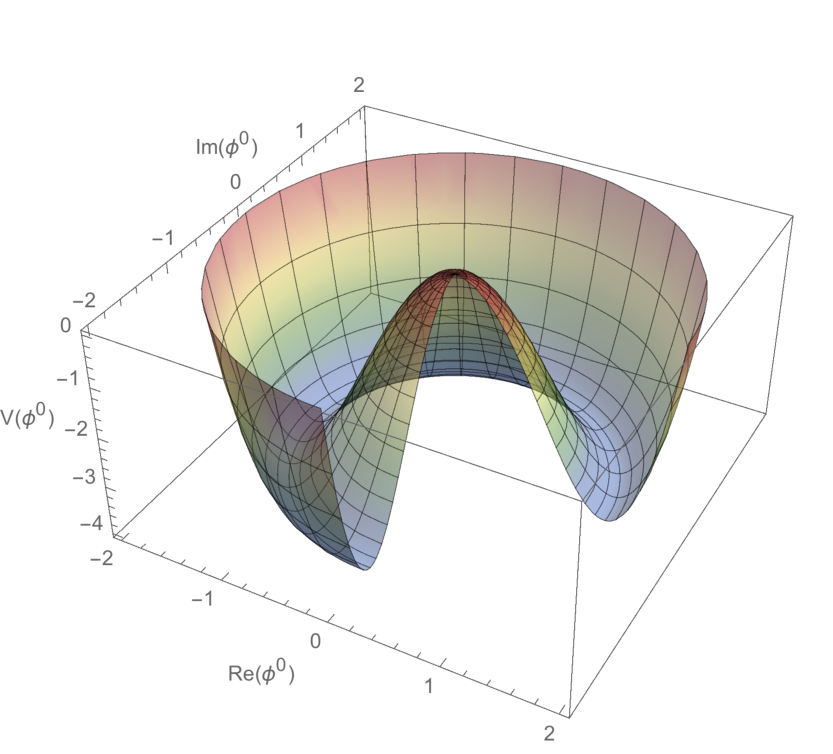
\includegraphics[width=0.9\textwidth]{IntroFigures/HiggsPotential.pdf}
 \caption{The shape of the Higgs potential (``Mexican hat''). The
   degeneracy of the potential is observed along the azimuthal angle\label{fig:MexHat}}
\end{figure}

where $U(x)$ is a unitary transformation that transforms the field
into the degenerate solution. An important consequence is that the
\textit{vev} of field preserves a $U(1)$ symmetry from the original
$\mathrm{SU(2)_{L}}\times U(1)_{\mathrm{Y}}$ symmetry of the
Lagrangian. Therefore the full electroweak symmetry of the SM
($\mathrm{SU(2)_{L}}\times U(1)_{\mathrm{Y}}$) is spontaneously broken
to $U(1)_{\mathrm{EM}}$.

This spontaneous breaking of the $\mathrm{SU(2)_{L}}\times
U(1)_{\mathrm{Y}}$ symmetry is responsible for the appearance of
masses to 3 of the four gauge bosons in the electroweak sector, this
is called: the Higgs mechanism. The masses become apparent when
replacing the \textit{vev} into the Higgs kinetic term in the
Lagrangian:

\begin{equation}
\label{eq:HiggsMass}
(D^{\mu}\Phi)^{\dagger}(D^{\mu}\Phi) \rightarrow
\Delta\mathcal{L} = \frac{1}{2}\begin{pmatrix} 0 & v\end{pmatrix} (gA_{\mu}^{a}\tau^{a} + g^{\prime}B_{\mu})(gA^{b\mu}\tau^{b} +g^{\prime}B^{\mu}) \begin{pmatrix} 0\\
  v\end{pmatrix}.
\end{equation}

Evaluating the matrix products, using $\tau^{a}=\sigma^{a}/2$ and
$\left\{\tau^{a},\tau^{b}\right\} = \delta^{ab}/2$, we find

 
\begin{equation}
\label{eq:HiggsMass2}
\Delta\mathcal{L} = \frac{\mathit{v}^{2}}{8}\left[g^{2}(A^{1}_{\mu})^2
  +g^{2}(A^{2}_{\mu})^2 + (-gA^{3}_{\mu}+g^{\prime}B_{\mu})^2)\right].
\end{equation}

This forms the mass matrix squared for the gauge boson in the
$(A^{i}_{\mu}, B_{\mu})$ basis
\begin{equation}
\label{eq:HiggsMass}
m^{2} = \left(\frac{v}{2}\right)^{2}
\begin{pmatrix} g^{2} & 0 & 0 & 0\\
0 & g^{2} & 0 & 0\\
0 & 0 & g^{2} & -gg^{\prime}\\
0 & 0 & -gg^{\prime} & g^{2}\\
\end{pmatrix},
\end{equation}

by diagonalizing this matrix, it is clearly observed that there are three
massive and one massless gauge boson, the linear combination of the
gauge fields and their respective masses are the following:

\begin{equation}
 \begin{aligned}
       &W^{\pm}_{\mu} = \frac{1}{\sqrt{2}}(A^{1}_{\mu}\mp A^{2}_{\mu})
        \qquad \text{with mass}  \qquad  m_{W} = g\frac{v}{2}\\
        & 
        Z^{0}_{\mu} = \frac{1}{\sqrt{g^{2}+g^{\prime
              2}}}(gA^{3}_{\mu}- g^{\prime 2}B_{\mu})
        \qquad \text{with mass}  \qquad  m_{Z} = \sqrt{g^{2}+g^{\prime
            2}}\frac{v}{2}\\
        &
        A_{\mu} = \frac{1}{\sqrt{g^{2}+g^{\prime
              2}}}(g^{\prime}A^{3}_{\mu}+ gB_{\mu})
        \qquad \text{with mass}  \qquad  m_{A} = 0
       \end{aligned}
\label{eq:BosonMasses}
\end{equation}

Besides providing the Higgs mechanism, the inclusion of the
$SU(2)_{L}$ field in the SM predicts the presence of a
self-interacting massive spin-0
boson, this is realized by the fluctuation of the field around the
\textit{vev}, i.e.
\begin{equation}
\Phi = \frac{1}{\sqrt{2}}\begin{pmatrix} 0\\
  v + h(x)\end{pmatrix},
\end{equation}
 
now collecting the higgs-related terms in the Lagrangian, we obtain
the following:

\begin{equation}
\mathcal{L}_{\mathrm{Higgs}} \supset
\frac{1}{2}\left(\partial_{\mu}h\right)^{2} -\lambda v^{2}h^{2} -
\lambda vh^{3} - \frac{\lambda}{4}h^{4}.
\end{equation}

Where the first term is the standard kinetic term, the second term is
the mass term ($m_{h} = \sqrt{2\lambda}v$), and the last two are the higgs self-interaction terms. 
\section{Fermion Masses}\label{yukawa}
Fermion masses in the standard model arise from the inclusion of
interaction terms between the fermions and the $\Phi$ field~\cite{WeinbergLeptons}, when
the latter is at the \textit{vev}. These interactions are called
Yukawa terms, they have different strength depending on the particle
type and generation. The corresponding part of the Lagrangian in
Eq.~\ref{eq:theSMlagrangian} is
\begin{equation}
\label{eq:yukawa}
\mathcal{L}_{Yukawa} = -y_{e}\bar{\ell}_{L}\Phi e_{R} - y_{u}\bar{q}_{L}\Phi u_{R}  -
y_{d}\bar{q}_{L}\tilde{\Phi} u_{d} + (h.c),
\end{equation}

where $y_{e,u,d}$ are the Yukawa couplings to the leptons, up-type
quarks, and down-type quarks, respectively; $\tilde{\Phi} =
i\sigma^{2}\Phi^{*}$ with weak hyper-charge $Y = -1/2$ is used in the
third term to generate the down-type quark masses. After the $\Phi$
field acquires its \textit{vev} we can identify the fermion mass terms
as

\begin{equation}
 \begin{aligned}
       &m_{e} = \frac{y_{e}v}{2}  \qquad m_{u} = \frac{y_{u}v}{2}  \qquad  m_{\mu} = \frac{y_{d}v}{2} \\
       &m_{\mu} = \frac{y_{\mu}v}{2}  \qquad m_{c} = \frac{y_{c}v}{2}
       \qquad  m_{s} = \frac{y_{s}v}{2} \\
       &
       m_{\tau} = \frac{y_{\tau}v}{2}  \qquad m_{t} = \frac{y_{t}v}{2}  \qquad  m_{b} = \frac{y_{b}v}{2}.
       \end{aligned}
\label{eq:BosonMasses}
\end{equation}

The Yukawa terms give mass to all the fermions in the SM, provide decay modes of the physical higgs boson -- with
$h\rightarrow b\bar{b}$ having the highest branching fraction --, and
allow the fermions to modify the observed mass of the Higgs boson through
loop corrections -- the most important correction comes from the
top-quark, which has the largest Yukawa coupling.
\section{On the Hierarchy Problem and Supersymmetry}
A concrete example of the limitations of the SM is the apparent
``unnatural'' value of the Higgs boson mass~\cite{CMSHIGGS,ATLASHIGGS}
($m_{H} \approx 125\GeV$). This can be understood by looking at the
physical Higgs mass after the fermionic quantum corrections are applied. Since the Yukawa coupling of the top
quark is the largest, we concentrate on it. The physical mass of the
Higgs ($m_{h^{0}}$) is 
\begin{equation}
\label{eq:higgMass}
m^{2}_{h^{0}} = m^{2}_{h^{0}(\mathrm{bare})} + \Delta m^{2}_{h^{0}}
\end{equation}

\begin{fmffile}{test2}
\begin{equation}
 \begin{aligned}
       \Delta m^{2}_{h^{0}} &= \hspace{0.9cm}
\begin{gathered}
\begin{fmfgraph*}(50,33)\fmfkeep{fermion1}
\fmfleft{i} \fmfright{o} \fmf{dashes}{i,v1} \fmf{dashes}{v2,o}
\fmflabel{$h^{0}$}{i}
\fmflabel{$h^{0}$}{o}
\fmf{plain,left, label=$t$,tension=.3}{v1,v2,v1}
\end{fmfgraph*}
\end{gathered} \hspace{0.9cm} + \cdots\\
        & =  \hspace{1.2cm}-\frac{3|y_{t}|^{2}}{8\pi^{2}}\Lambda^{2}_{\mathrm{UV}} \hspace{0.7cm}+ \cdots,
       \end{aligned}
\label{eq:HiggsMassCorrection}
\end{equation}
\end{fmffile}

where $m_{h^{0}(\mathrm{bare})}$ is the mass of the Higgs without
quantum corrections, $\Delta m^{2}_{h^{0}}$ is the contribution from
quantum corrections to the Higgs mass squared, and $\Lambda_{\mathrm{UV}}$
is the ultra violet cuttoff of the theory. If the SM is indeed a
complete theory, then we expect $\Lambda_{\mathrm{UV}} \sim
M_{\mathrm{planck}} \sim 10^{19}\GeV$, where gravity becomes
relevant. The later implies that the observed Higgs mass ($\approx
$125\GeV) is obtained by a remarkable cancelation between the two terms
in the right-hand side of equation~\ref{eq:higgMass}, this fine
tunning has become to be known as the hierarchy problem or the
naturalness problem of the Higgs mass. A possible alleviation of this problem in the
introduction of new physics a mass scale in between the weak scale
($\sim$ 100\GeV) and the Planck scale. As mentioned earlier, one
appealing theory is supersymmetry, since besides alleviating the
naturalness problem, it also provides unification of the gauge coupling at
about $M_{\mathrm{planck}}$ and a suitable dark matter candidate. In
supersymmetric theories there is a new particle for every field degree
of freedom in the SM, the new particles have the opposite
spin-statistics to those of the SM, i.e. bosons in the SM have fermion
partners in supersymmetric models and vice versa. The scalar partners
of the SM fermions are commonly known as sfermions (squarks, sleptons,
etc.) and they are labeled with as their SM counterparts but adding a
tilde (e.g. $\tilde{t}, and \tilde{e}$  for the stop, and selectron,
respectively).

Supersymmetry alleviates the naturalness problem by adding new quantum
corrections to the Higgs mass, again the most relevant contribution
comes from the top partners (two of them) which contribute with an opposite sign
to the Higgs mass radiative corrections due to their bosonic nature:\\\\
\begin{fmffile}{test2}
\begin{equation}
 \begin{aligned}
       \Delta m^{2}_{h^{0}} &= \hspace{0.9cm}
\begin{gathered}
\begin{fmfgraph*}(50,33)\fmfkeep{fermion}
\fmfleft{i} \fmfright{o} \fmf{dashes}{i,v1} \fmf{dashes}{v2,o}
\fmflabel{$h^{0}$}{i}
\fmflabel{$h^{0}$}{o}
\fmf{plain,left, label=$t$,tension=.3}{v1,v2,v1}
\end{fmfgraph*}
\end{gathered} \hspace{0.9cm} + \hspace{0.9cm} \begin{gathered}
\begin{fmfgraph*}(50,33)\fmfkeep{boson1}
\fmfleft{i} \fmfright{o} \fmf{dashes}{i,v1} \fmf{dashes}{v2,o}
\fmflabel{$h^{0}$}{i}
\fmflabel{$h^{0}$}{o}
\fmf{dashes, left, label=$\tilde{t}_{i}$,tension=.3}{v1,v2,v1}
\end{fmfgraph*}
\end{gathered} \hspace{0.9cm}+ \hspace{0.9cm} \begin{gathered}
\begin{fmfgraph*}(50,33)\fmfkeep{boson2}
\fmfleft{i} \fmfright{o} \fmf{dashes}{i,v1} \fmf{dashes}{v1,o}
\fmflabel{$h^{0}$}{i}
\fmflabel{$h^{0}$}{o}
\fmf{dashes, right, label=$\tilde{t}_{i}$,tension=.7}{v1,v1}
\end{fmfgraph*}
\end{gathered}\hspace{0.9cm} + \cdots\\\\
        & =
        \hspace{1.1cm}-\frac{3|y_{t}|^{2}}{8\pi^{2}}\Lambda^{2}_{\mathrm{UV}}
        \hspace{0.5cm}+\hspace{0.9cm} 2\frac{3|y_{t}|^{2}}{16\pi^{2}}\Lambda^{2}_{\mathrm{UV}}
        -\sum^{2}_{i}\frac{3|y_{t}|^{2}m^{2}_{\tilde{t}_{i}}}{8\pi^{2}}\mathrm{log}\left(\frac{\Lambda_{\mathrm{UV}}}{m_{\tilde{t}_{i}}}\right)
        \hspace{0.35cm} + \cdots\\\\
        \Delta m^{2}_{h^{0}} &= -\sum^{2}_{i}\frac{3|y_{t}|^{2}m^{2}_{\tilde{t}_{i}}}{8\pi^{2}}\mathrm{log}\left(\frac{\Lambda_{\mathrm{UV}}}{m_{\tilde{t}_{i}}}\right)
        + \cdots,\\
       \end{aligned}
\label{eq:HiggsMassCorrection2}
\end{equation}
\end{fmffile}

where $m_{\tilde{t}_{i}}$ is the mass of the $ith-$stop. As it can be
seen in Equation~\ref{eq:HiggsMassCorrection2} the additional quantum
corrections due to the inclusion of the stop loops cancel the
quadratic divergence of the top
quark contribution, but they add a logarithmic dependence -- that is
why the naturalness problem is only alleviated. By requiring natural supersymmetric
scenario, where the fine tuning is at the 10\% level, requires
$m_{\tilde{t}_{i}} < 400\GeV$, which in turn has motivated various LHC
searches since stop production cross-sections at that mass level is
high enough to be detected.

The particle spectra of SUSY is rich, and one important component comes
from spin-1/2 particles that are the partners of the SM vector bosons,
these particles are known as gauginos. Similar to the mixing of the
$\mathrm{SU(2)\times U(1)}$ gauge boson the gauginos, including the
higgsino (also a spin-1/2), mix to form neutral and charged
eigenstates, particularly, there are two neutral mass eigenstates (the
neutralinos) $\tilde{\chi}^{0}_{1,2}$, and two charged  mass eigenstates (the
charginos) $\tilde{\chi}^{\pm}_{1,2}$. In most models the lightest neutralino
($\chi^{0}_{1}$) is the lightest supersymmetric mass state.

In order to explain the observed life time of the proton supersymmetric
model usually require an extra symmetry (R-parity) -- which is not
built in in the theory --  that is conserved,
\begin{equation}
\label{eq:rparity}
R = (-1)^{3(\mathrm{B}-\mathrm{L}) + 2s},
\end{equation}

where B is the baryon number, L is the lepton number, and s is the spin
of the particle. By construction all SM particle are even (R=+1), and
all SUSY particles are odd (R=-1) under R-parity. This multiplicative
quantum number has very interesting experimental consequences: 1) the
supersymmetric particles are produce in even numbers (usually) at
particle colliders, 2) supersymmetric particles decay to an even number
of  supersymmetric particles, and 3) the lightest supersymmetric
particle is stable
-- in fact this last point is a consequence of the second. The later
consequence in conjunction with the fact that in most SUSY model the
lightest particle in the spectra in neutral, provides a good weakly
interaction dark matter candidate. 

Since SUSY particles couple to the Higgs boson -- as they help to
alleviate the naturalness problem -- it is expected for some of them
to produce decays involving Higgs final states, such as
$\tilde{q}\rightarrow h^{0}\chi^{0}$ and
$\tilde{\chi}^{2}_{0}\rightarrow h^{0}\tilde{\chi}^{1}_{0}$, that
could enhance the SM prediction for Higgs production and could be
search for at the LHC (see Chapters~\ref{HggRazor}
and~\ref{hggPheno}). So far SUSY has not been detected but these final
states will certainly increase the discovery potential of the LHC experiments.
%\chapter{Supersymetry and Naturalness}
\chapter{Dark Matter and Weakly Interacting Particles}
Different measurements during the twentieth century indicate that
baryonic matter is not the dominant form of matter in the
universe. In fact, recent measurements constraint the amount of baryonic matter
to be about 5\% of the total energy density, while the rest is
comprise of dark matter and dark energy, accounting for approximately 27\%  and 68\% ,
respectively. The existence of dark matter has been inferred by
several astronomical and astrophysical measurements since the 1930s,
as well as the recent success of the standard model of Big Bang
cosmology (commonly known as the $\mathrm{\Lambda CDM}$). Nowadays,
the existence of dark matter is widely accepted but little is known
about its nature. Dark energy is perhaps the least understood component
of our Universe, currently, we infer its existence based on the
missing energy density in conjunction with the measured flatness of
the universe, as well as the accelerated expansion of the universe.

This chapter is intended to briefly summarize the evidence supporting
the existence of dark matter and to introduce the concepts needed to
understand the basis of the current searches for dark matter in direct
detection experiments, indirect detection experiments, and the
experiments at the Large Hadron Collider. The rest of this chapter has
been based on~\cite{Golwala,DM_Primer}.

\section{The Evidence for Dark Matter}
\subsection{Early evidence}
Perhaps the first convincing evidence of the existence of dark matter
was the measurements carried out in the Coma cluster by F. Zwicky in
1933 -- Oort also had measured earlier inconsistencies between the
velocities of stars near the galactic center and the luminous
mass. Zwicky measured the velocities of the galaxies in the cluster by observing the
doppler shifts in their emission spectra and by employing the virial
theorem he was able to calculate the cluster's total mass~\cite{zwikcy1,ZZZZW}. The cluster
mass was $M_{\mathrm{cluster}} = 4.5\times10^{13}M_{\odot}$, since
there are approximately 1,000 galaxies in the cluster the average
galatic mass is $M_{\mathrm{galaxy}} = 4.5\times10^{13}M_{\odot}$. The
mass of the galaxies were also measured using the standard
mass-to-light ratio which yielded a galactic mass approximately 2\% of
that measured by Zwicky. Therefore most of the mass in the Coma
cluster was missing, or at least did not interact electromagnetically
and thus dubbed ``dark matter''.

 In the 1970s Vera Rubin and others
set to measure the rotation curves of about 100 isolated
galaxies~\cite{rubin}. What they found was that the rotation
velocities reached a plateau at radii of about 10\unit{kpc}, which
blatantly contradicted the observations from the luminous matter
profile in the galaxies. The measured rotation curves measured by
Persic and Salucci~\cite{PandS} are shown in Figure~\ref{fig:rotationcurve}, and a
rotation curve from the spiral galaxy M33 is shown in
Figure~\ref{fig:M33}. The fact that the luminous matter decays
exponentially with the radius of the galaxy implies that  the velocity
of gas and stars in the outskirts of the galaxy should start to
decrease at around the optical radius $R_{\mathrm{opt}} = $10\unit{kpc} -- the radius
such that 83\% of the light is contained in it. As observed in
Figures~\ref{fig:rotationcurve} and~\ref{fig:M33}, this is not the case, since the
velocities tend to be flat or even increase as a function of the
galactic radius. To solve this conundrum one can introduce a dark
matter halo with an spherically symmetric profile to account for the
apparent missing mass that would explain the observed rotation
curves. The most pedagogical way to visualize this effect is by
considering the rotation velocity to be constant (at large radius),
assuming  circular trajectories in the galactic disk, and using a
spherically symmetric density profile. Thus one finds
\begin{equation}
\label{eq:densityProfile}
\begin{aligned}
       &\frac{GM(r)}{r^{2}} = \frac{\mathrm{v}^{2}_{c}}{r} 
        \qquad \text{and}  \qquad  M(r) = \int^{r}_{0} 4\pi \rho(r) r^{2}dr\\
        & 
        \Rightarrow \qquad \frac{\mathrm{v}^{2}_{c}r}{G} = 4\pi
        \int^{r}_{0} \rho(r) r^{2}dr \qquad \text{}\\
        & \Rightarrow \qquad \rho(r) = \frac{\mathrm{v}^{2}_{c}}{4\pi
          G r^{2}}\qquad \text{},
       \end{aligned}
\end{equation}

where $\rho(r)$ is the density profile of the dark matter halo,
$\mathrm{v}_{c}$ is the constant rotational velocity (about
220\unit{km/s}), $G$ is the gravitational constant, and $r$ is the
galactic radius. A more accurate density profile, which fits the
observed galaxy rotation data, was proposed by Navarro, Frenk, and
White~\cite{NFW}
\begin{equation}
\rho(r) = \frac{\rho_{0}}{\frac{r}{R_{s}}\left( 1+\frac{r}{R_{s}}\right)^{2}},
\label{eq:NFW}
\end{equation}
where the central density ($\rho_{0}$) and the scale radius ($R_{s}$)
are parameters that vary from galaxy to galaxy.

\begin{figure}
 \centering
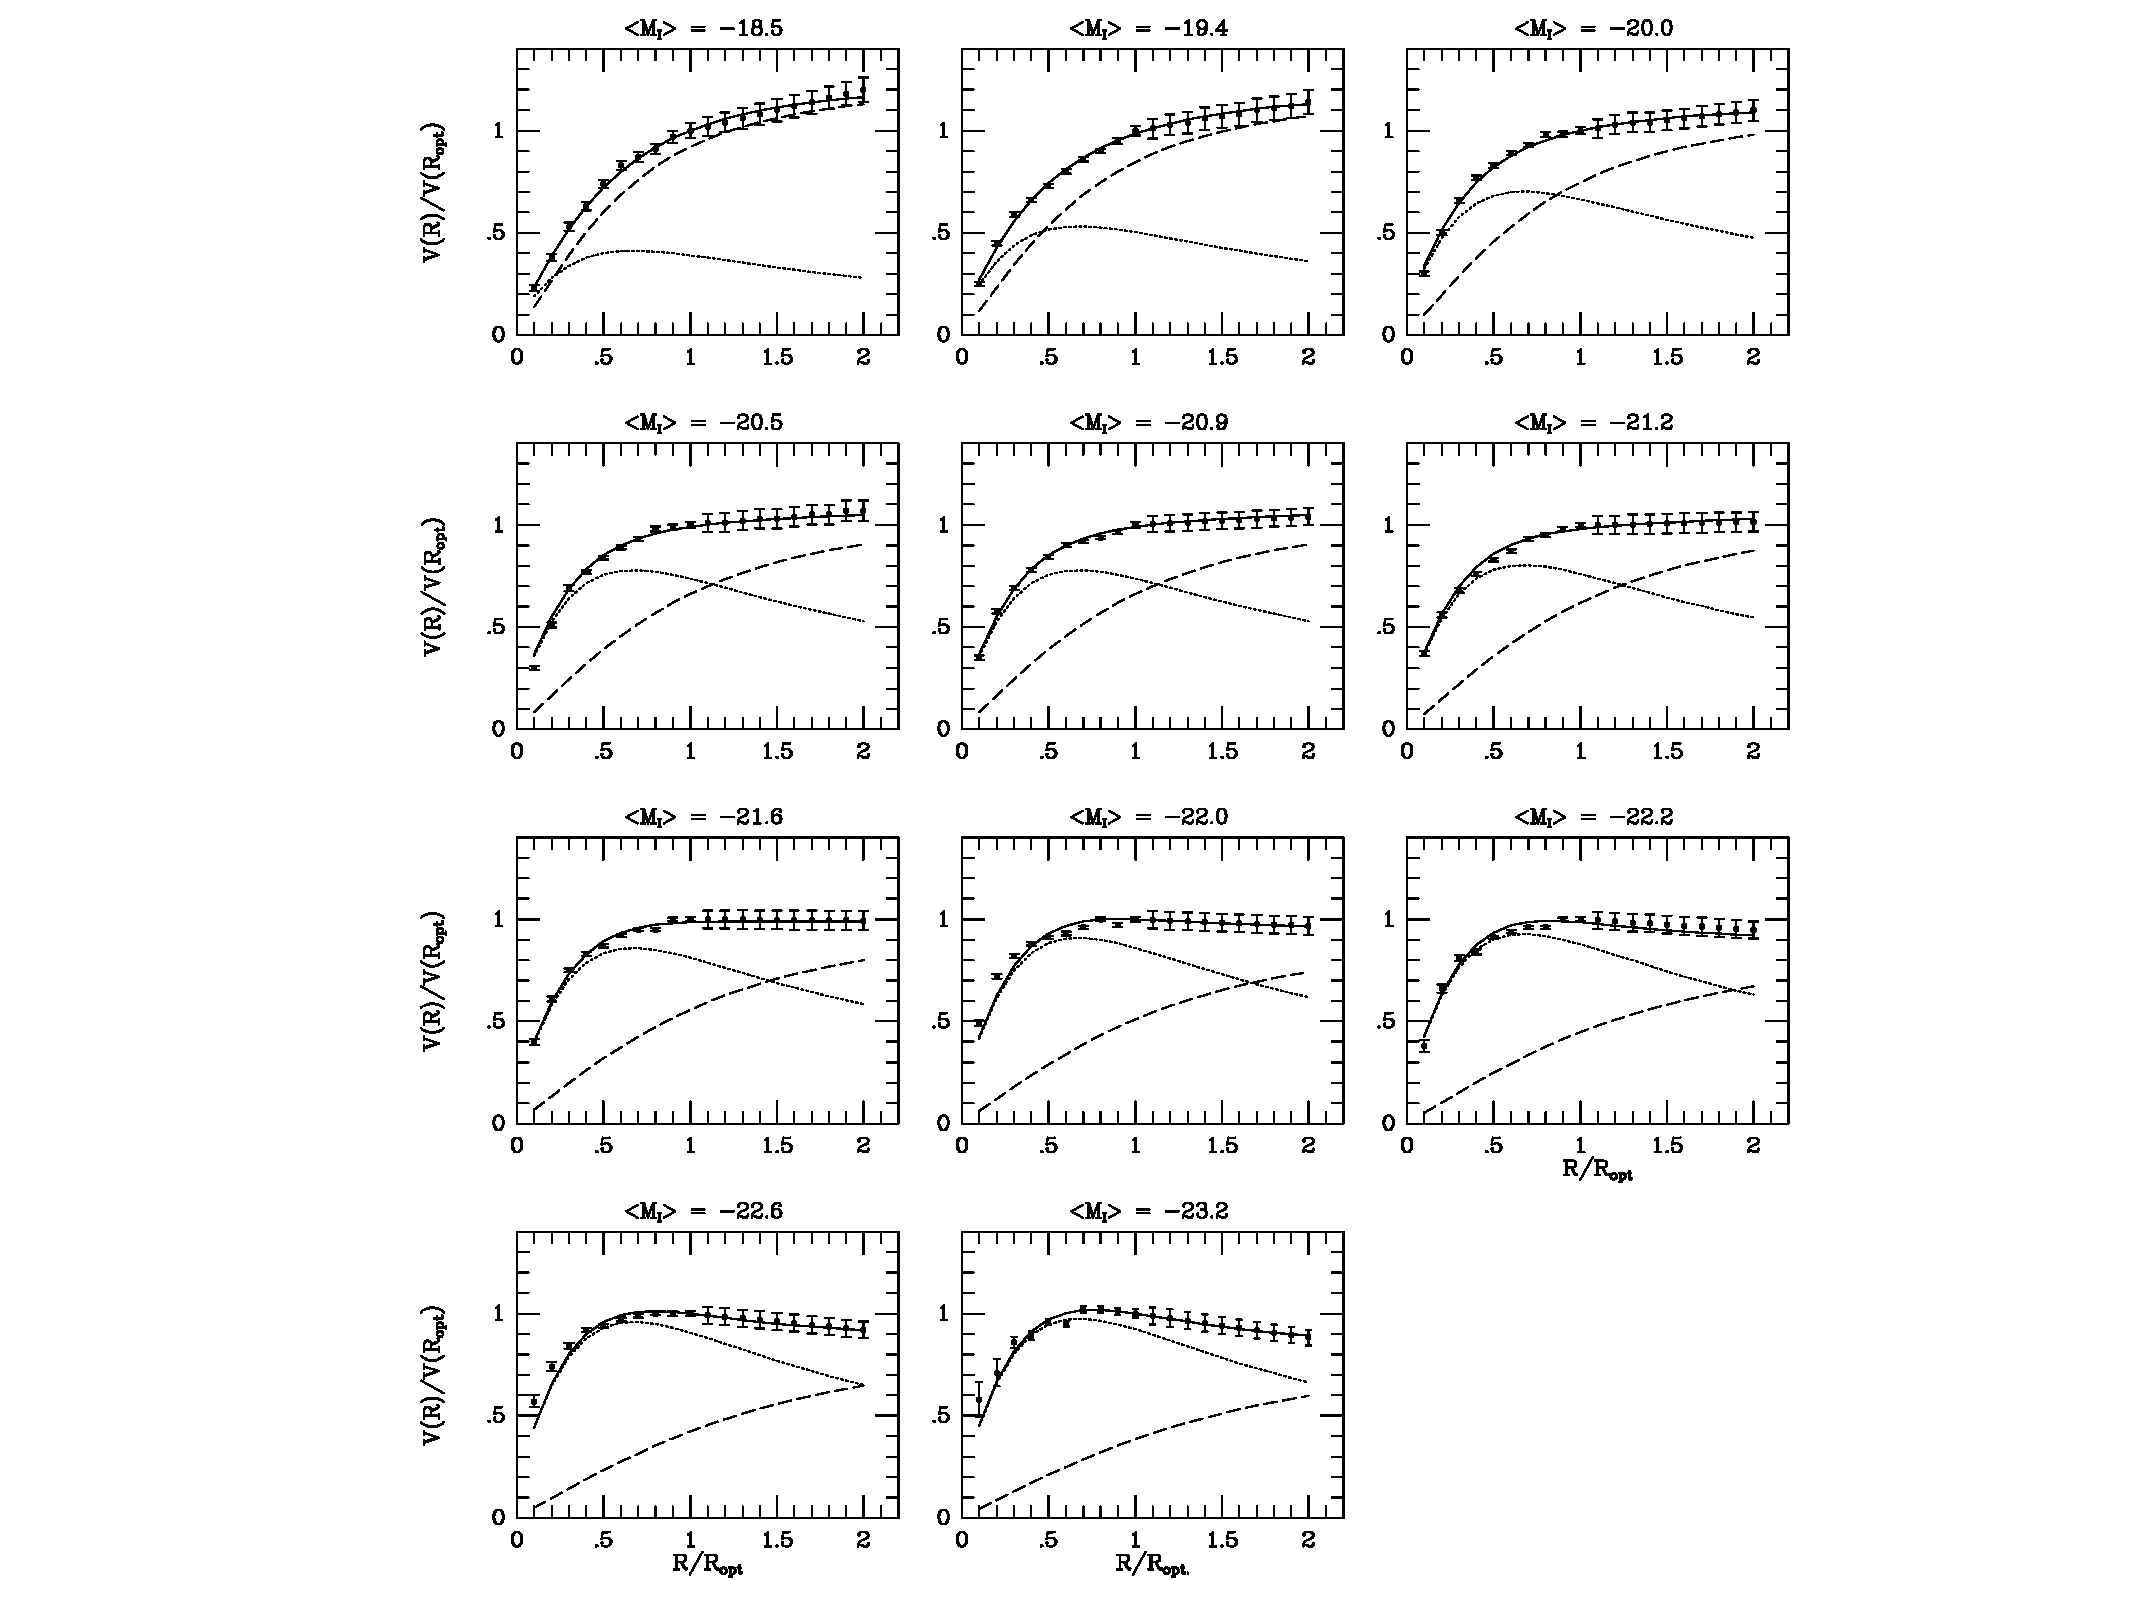
\includegraphics[width=0.7\textwidth]{IntroFigures/RotationCurve1.pdf}
 \caption{The rotation curves for different galaxies as measured by Persic and Salucci~\cite{PandS}.\label{fig:rotationcurve}}
\end{figure}
\begin{figure}
 \centering
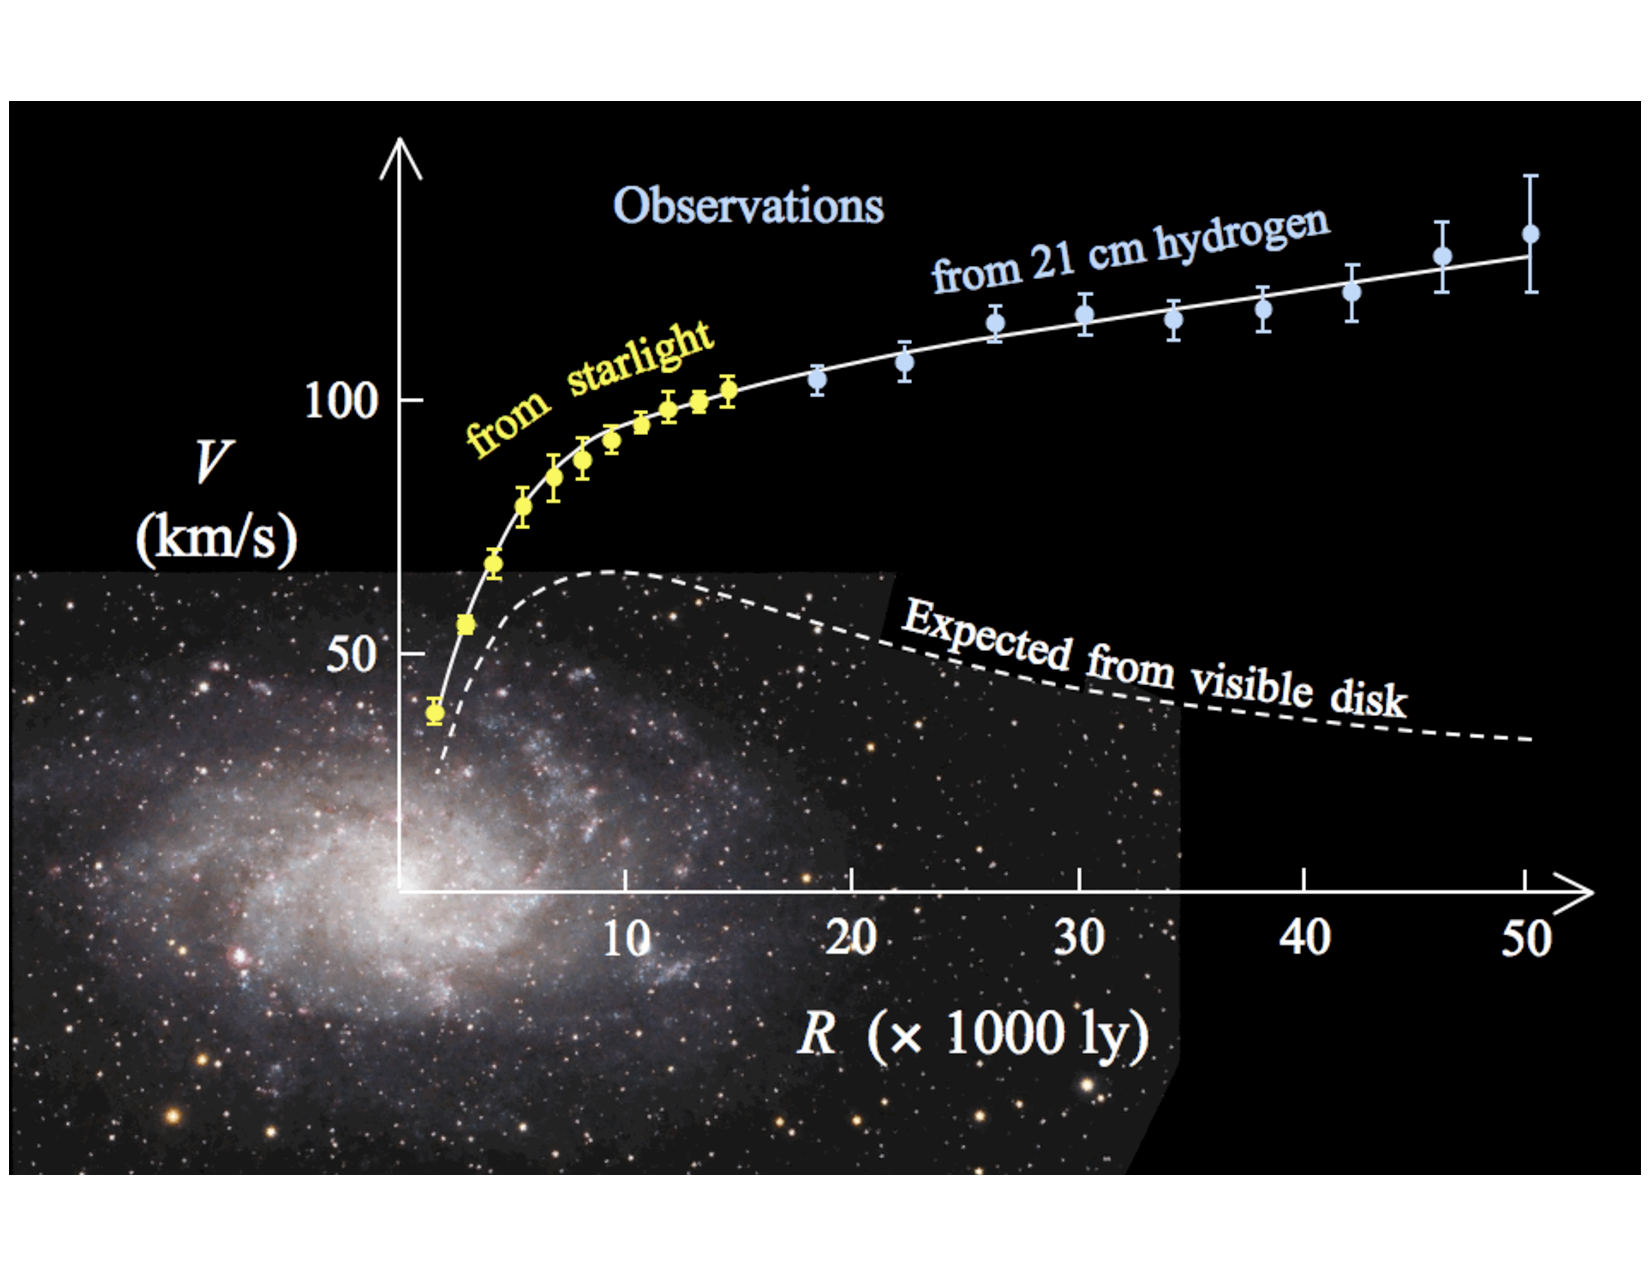
\includegraphics[width=0.7\textwidth]{IntroFigures/M33_rotation_curve_HI.pdf}
\caption{The rotation curve of the M33 galaxy.\label{fig:M33}}
\end{figure}

\subsection{Cosmological evidence}
Cosmological evidence arise later by comparing the measurements of light
elements (H, D, He, and Li) -- produced at
the early stages of the universe in what is called the Big Bang
Nucleosynthesis -- abundances with
the theoretical calculations of nuclear physics and known reaction
rates. The results are shown in Figure~\ref{fig:BBN}, where the colored
widths in the abundances represent the uncertainties in the calculations, the
rectangular boxes represent the experimental measurements, and the
vertical band indicates the region allowed by the deuterium
observation. R. H Cyburt calculated possible values of the baryon
relative density ($\Omega_{b}$) by using two deuterium measurements~\cite{BBN}
\begin{equation}
\label{eq:BBN}
\begin{aligned}
       &\Omega_{b}h^{2} = 0.0229\pm0.0013 
        \qquad \text{and}  \qquad  \Omega_{b}h^{2} = 0.0216^{+0.0020}_{0.0021},
       \end{aligned}
\end{equation}

where $h$ is the reduced Hubble parameter. Again, the baryon density
is found to be very low compared to the energy budget of the universe,
thus indicating the presence of dark matter -- and later, dark energy.
\begin{figure}
 \centering
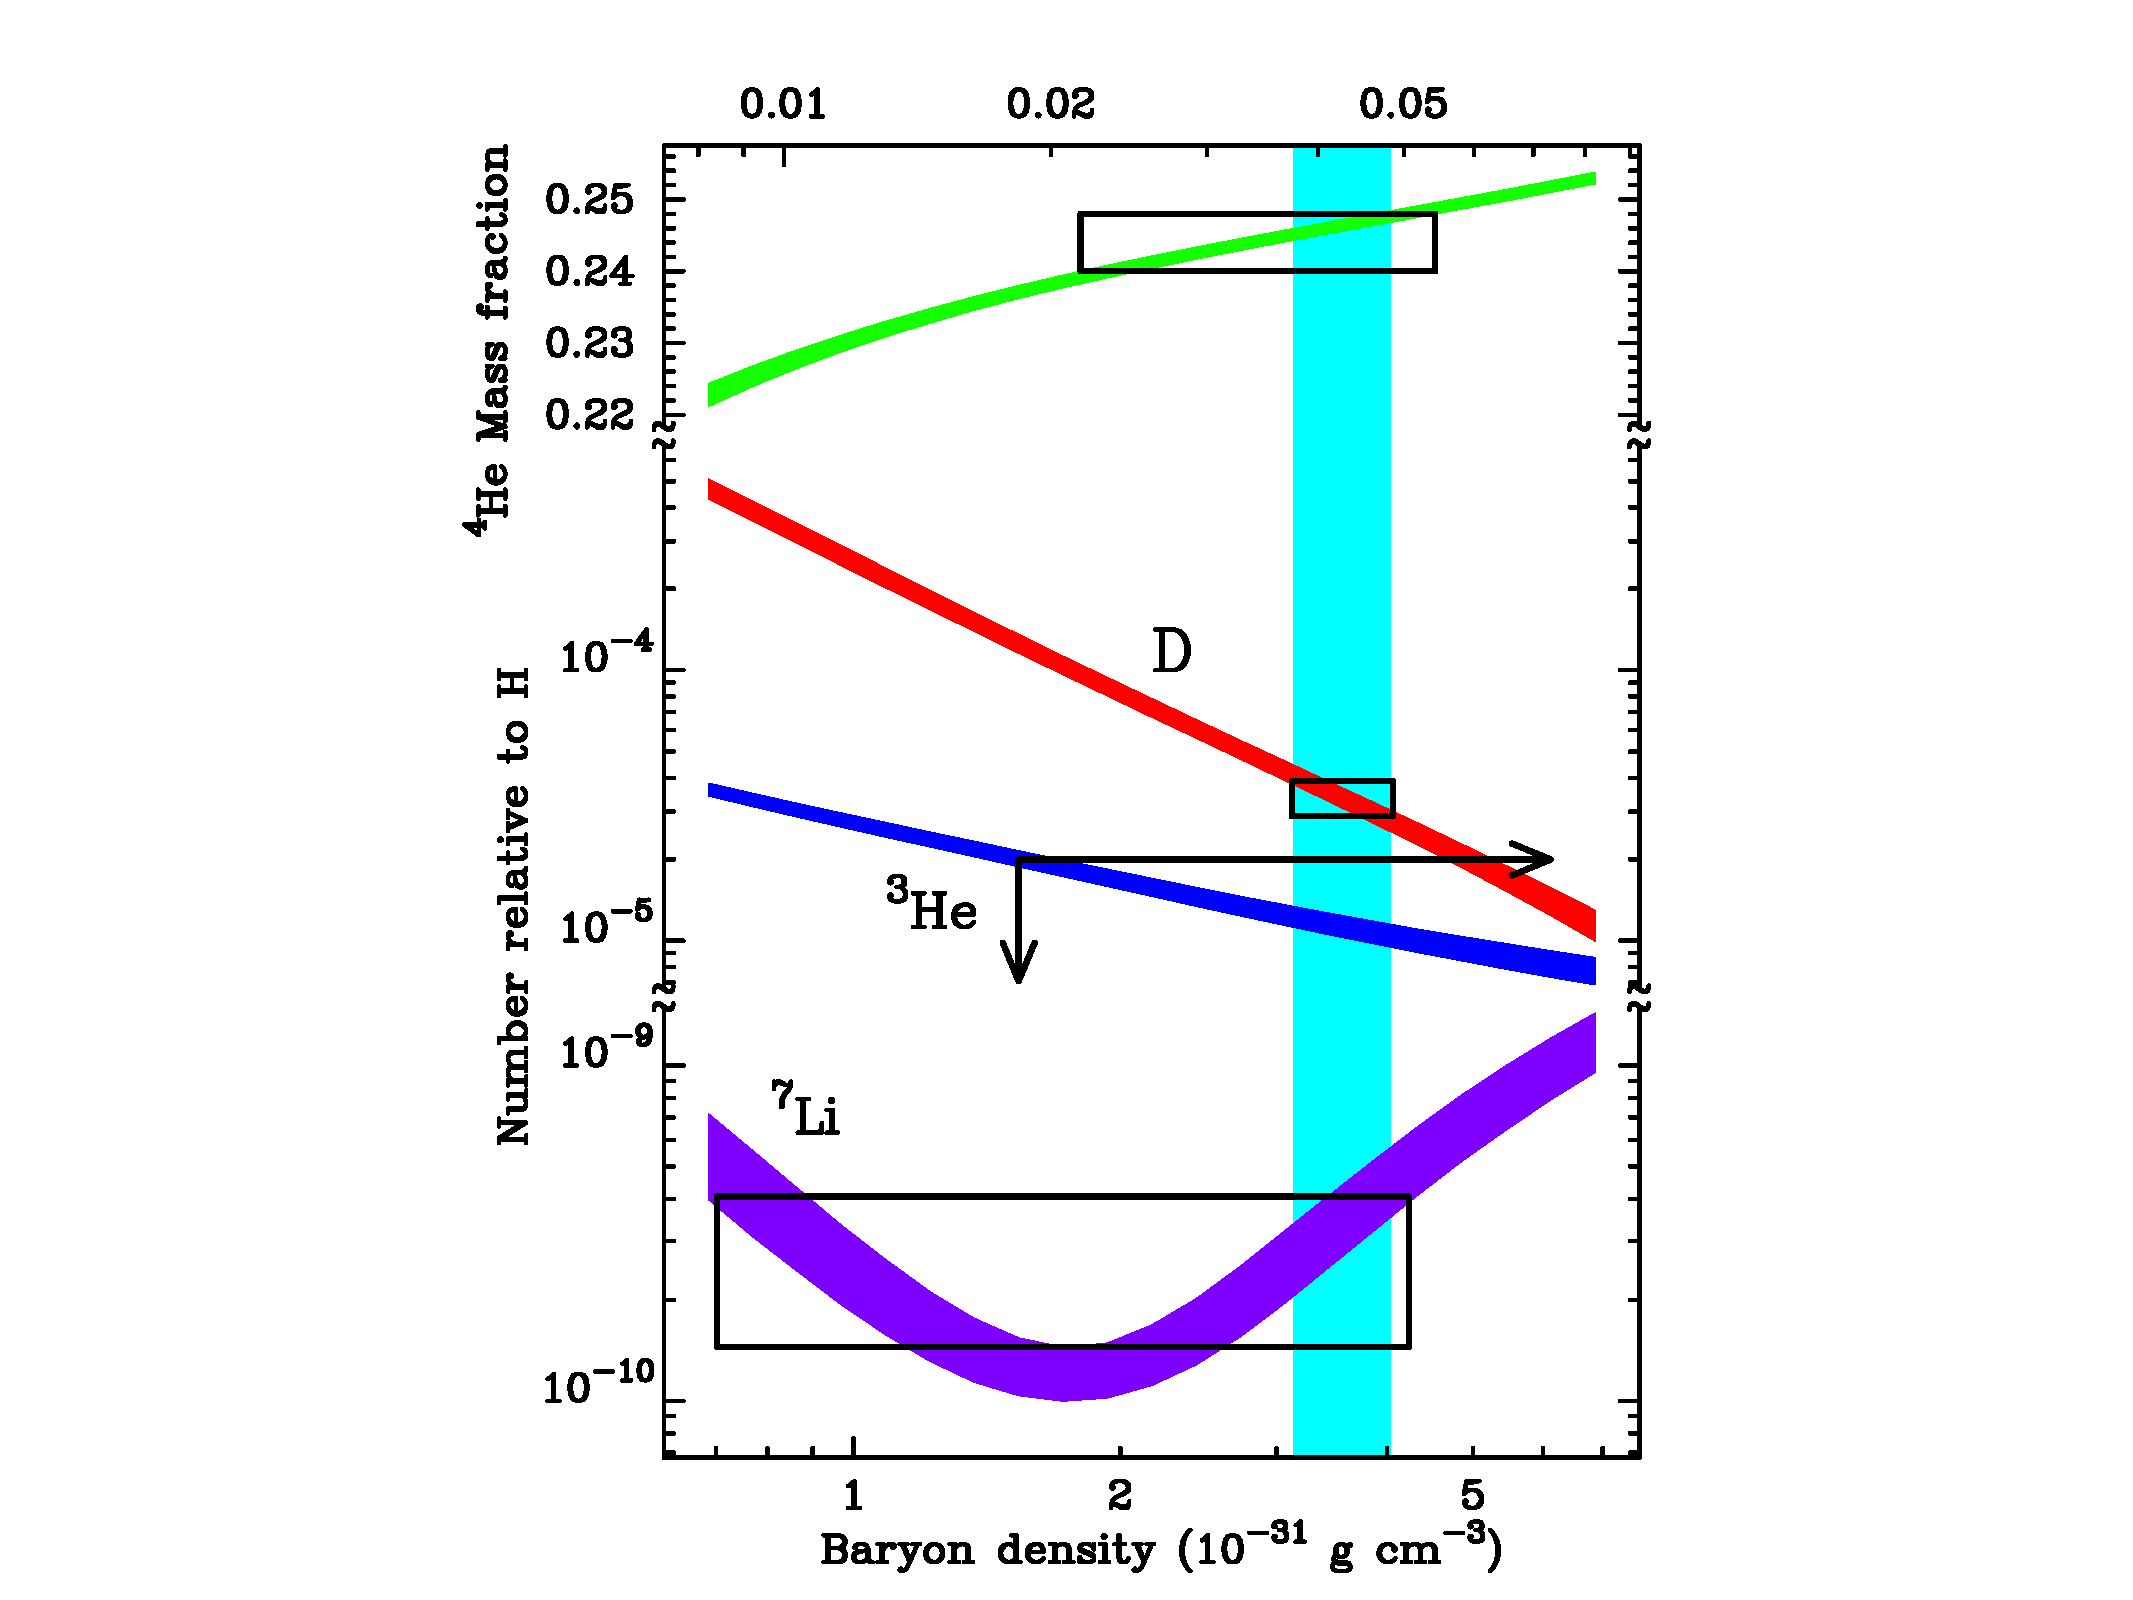
\includegraphics[width=0.6\textwidth]{IntroFigures/BBN.pdf}
\caption{BBN abundances as calculated by theory and measured by
  experiments in primordial-like areas of the universe with low
  concentration of Li.\label{fig:BBN}}
\end{figure}

The Cosmic Microwave Background (CMB) discovered by Penzias and Wilson
in 1964 as an excess of background temperature of about 3.5\unit{K} at a
wavelength of 7.5\unit{cm}~\cite{CMBDiscovery}, has undoubtedly
revolutionize the realm of precision cosmology. Later the CMB
has been measured to be consistent with an almost perfect black-body
spectrum with a temperature of  $2.72548\pm0.00057$\unit{K}, and thus
consistent with compatible with the expected relic radiation in the
form of photons from the epoch of recombination (380,000 years after
the Big Bang). Although, the CMB is very much isotropic and uniform, there are
fluctuation of about 1 part in 10$^{5}$ in the temperature of the CMB
as measured by the COBE satellite. These fluctuations are attributed
to two different effects, first, the Sachs-Wolfe effect: where photons
with lower energy today came from denser areas at the time of
recombination as they lost energy on their way out (these are
associated with large angular scales). Second, the acoustic
oscillations of the photon-baryon fluid that underwent compression and
rarefaction and thus imprinted temperature fluctuations in the
photons released when the baryons became electrically neutral and the
CMS photons were released (these fluctuation are associated with small
angular scales). The Wilkinson Microwave Anisotropy Probe (WMAP)
measured the temperature fluctuations in the CMB with unprecedented
precision and allowed the measurement of different cosmological
parameters including the density of baryonic dark matter. The
spectrum of the CMB anisotropies is shown in
Figure~\ref{fig:CMBAnisotropies}, where a multipole expansion has been
performed in order to clearly see the intensity of each mode. The
features of CMB anisotropies are directly related to the cosmological
parameters such as baryonic matter and dark matter, this is clearly
shown in Figure~\ref{fig:CMBAnisotropies}, where different values of
the baryonic density are overlaid with the real data from WMAP; as
observed, the incorrect baryonic density clearly mismodels the
observations. Finally a global fit can be performed to the CMP power
spectrum and thus obtain the cosmological parameters. The Plank
satellite -- current state of the art CMB experiment --  has measured
the  relative densities to be~\cite{plank}
\begin{equation}
\label{eq:plank}
\begin{aligned}
       &\Omega_{b}h^{2} = 0.02230\pm0.00014
        \qquad \text{and}  \qquad  \Omega_{DM}h^{2} = 0.1188\pm0.0010\\
        &\Omega_{m}= 0.6911\pm0.0062
        \qquad \text{and}  \qquad  \Omega_{\Lambda} = 0.3089\pm0.0062,
       \end{aligned}
\end{equation}

where $\Omega_{DM}$ is the dark matter relative density, $\Omega_{m}$
is the total matter density (baryonic and dark), and
$\Omega_{\Lambda}$ is the dark energy relative density.
\begin{figure}
 \centering
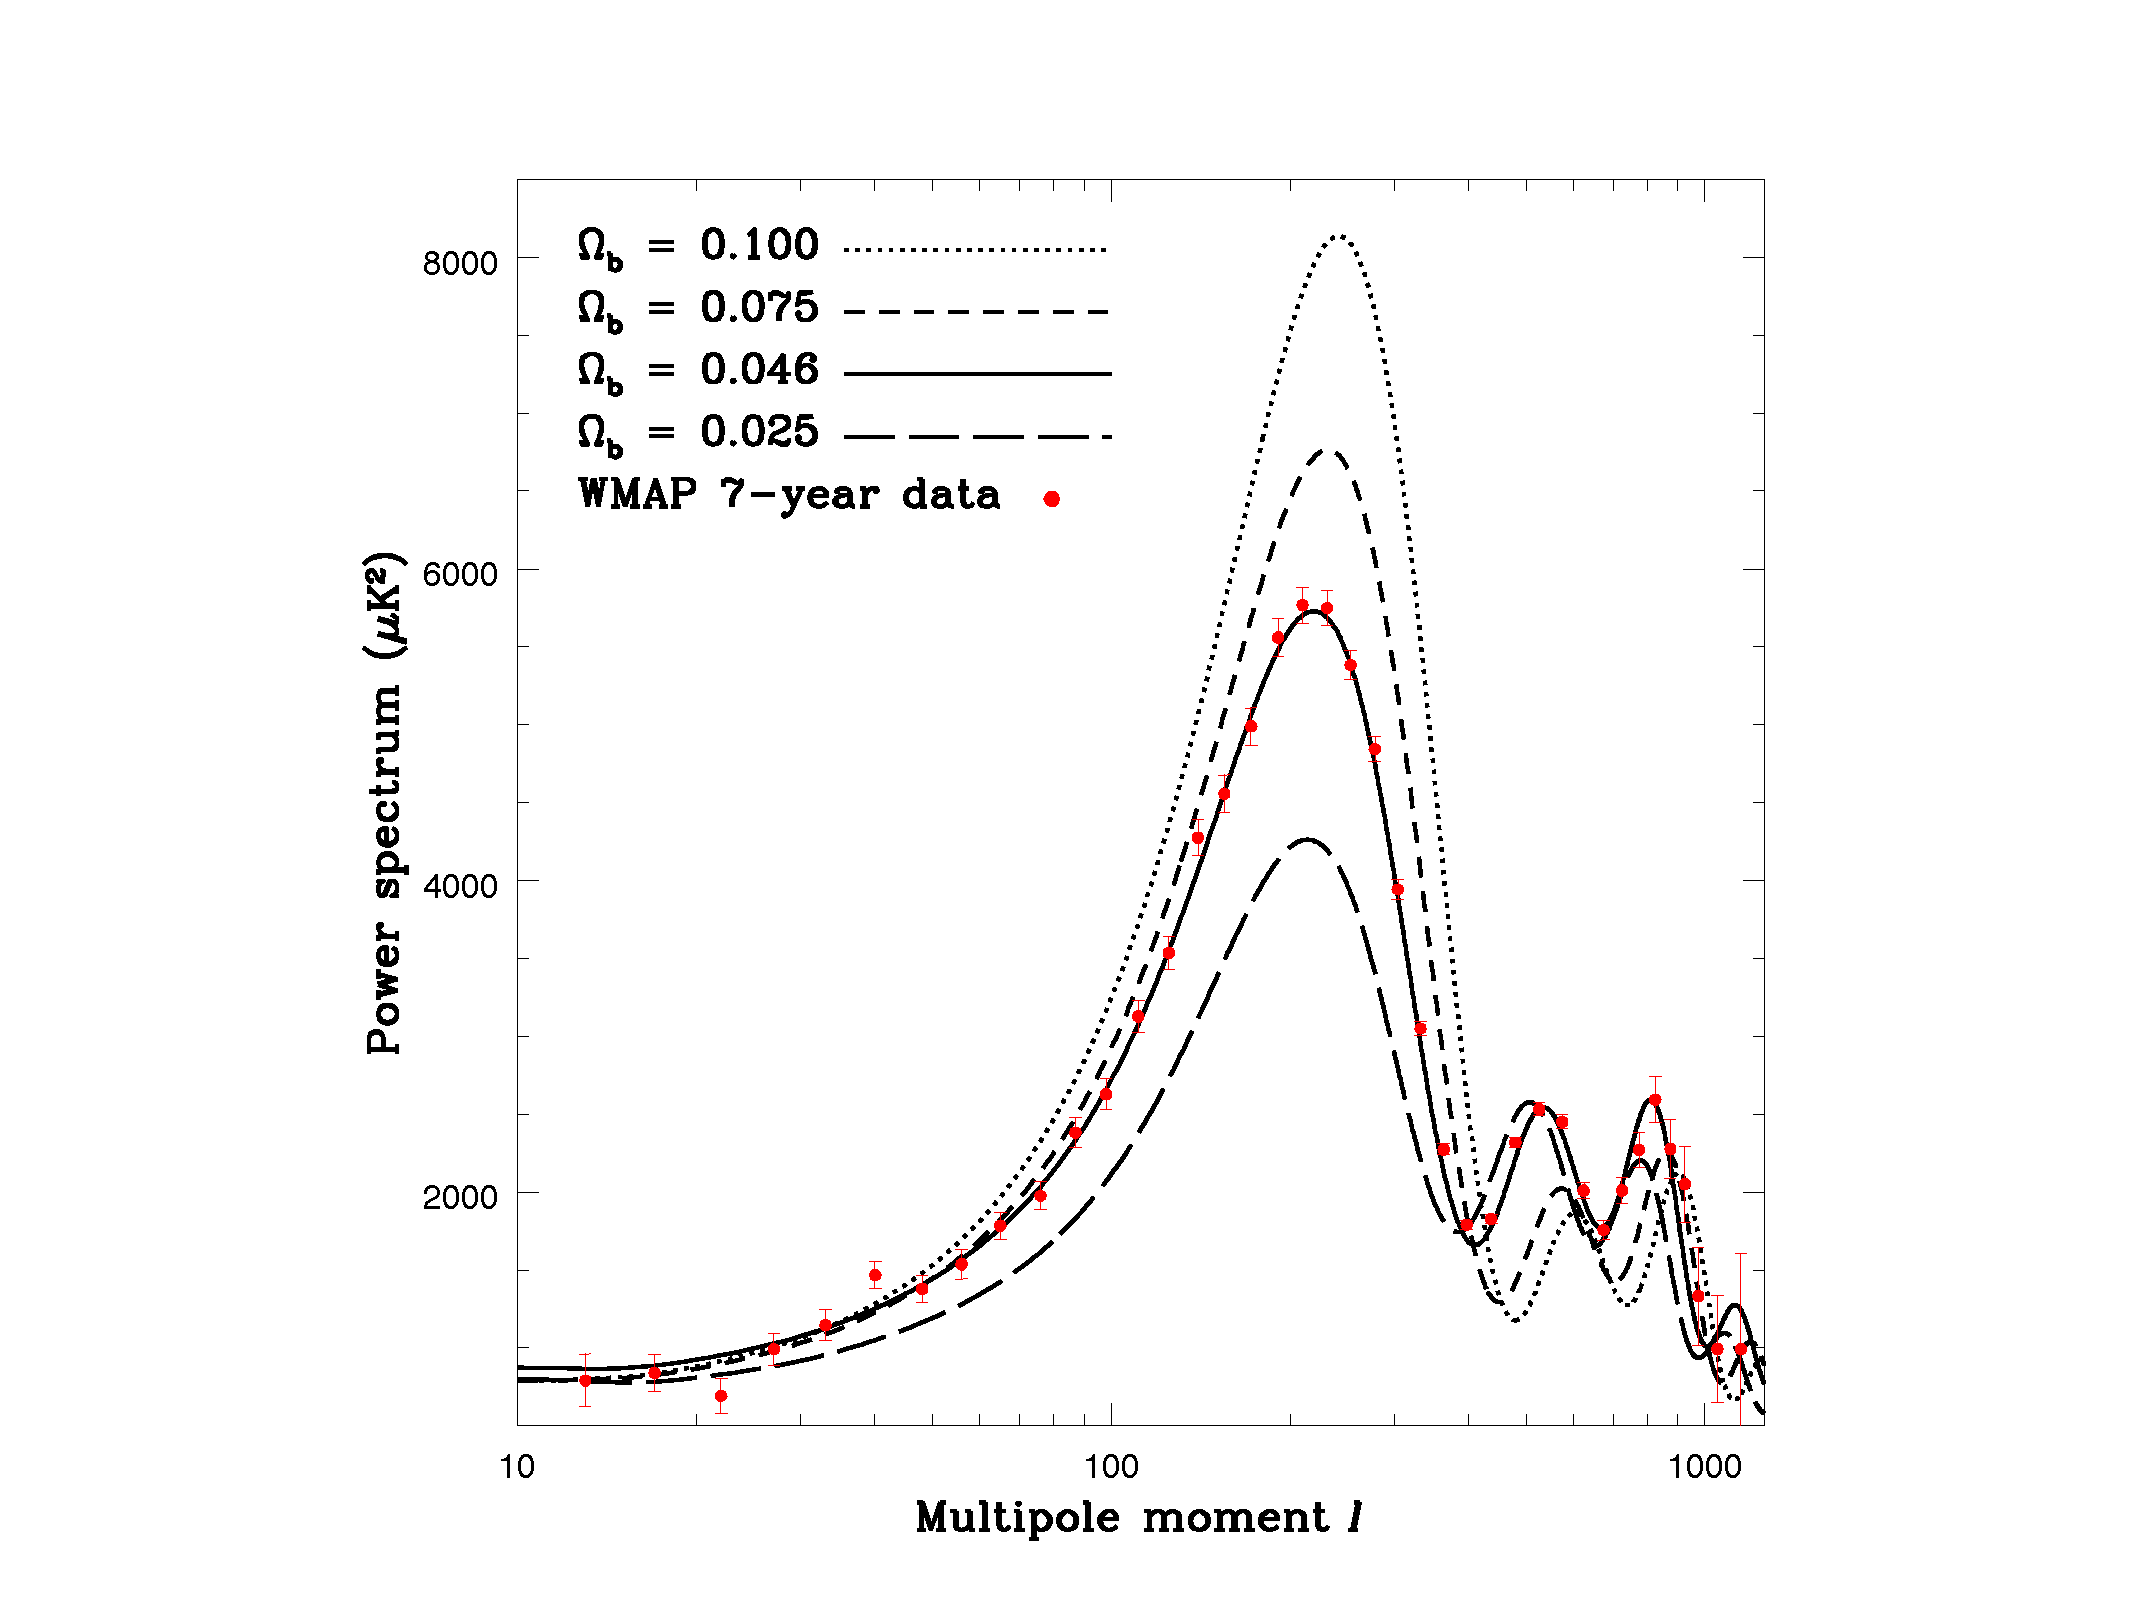
\includegraphics[width=0.7\textwidth]{IntroFigures/CMB_Multipole.pdf}
\caption{The CMB anisotropy spectrum measured by WMAP. Different
  values of the baryonic matter are also shown with different
  curves. In the multipole expansion of the CMB anisotropies
  $l\approx\pi/\theta$, where $\theta$ is the angular scale in radians.\label{fig:CMBAnisotropies}}
\end{figure}
\subsection{Recent evidence}

Most recent evidence for dark matter was obtained from the Bullet
cluster, formed by the sub-cluster (``the bullet'') colliding with the
larger cluster 1E 0657-56. During the collision, the galaxies pass by
each other without interacting since the inter-galaxy distance is
about 1\unit{Mpc}. Nevertheless, the bulk of the baryonic mass in the cluster is
formed by the hot intergalactic gas that did interact during the
collision, the excitations in the gas produced X-rays that were
detected by the Chandra X-ray Observatory. This measurement provides
an approximate distribution of the baryonic mass in the Bullet cluster
that was compared with measurements carried out by using weak
gravitational lensing. The comparison revealed that regions from
where the detected X-rays originated did not match the regions
compatible with gravitational lensing measurements, in fact the
majority of the cluster's mass is non-baryonic in nature~\cite{bullet}. Similar
measurements have been recently made with the Hubble Space Telescope~\cite{RingDM}.

\section{Weakly Interacting Dark Matter Candidates}
There are several dark matter suitable dark matter candidates, such as
axions, MACHOs, Kaluza-Klein particles, among others. Nevertheless, the most relevant DM candidate for this
thesis is what is called a Weakly Interacting Massive Particle
(WIMP). WIMPs are perhaps the most widespread non-baryonic DM
candidate since they have compelling properties, including the
prediction of the correct abundance of dark matter that we observe
today as a relic from
the early stages of the universe. Besides their gravitational
interaction, WIMPs only interact with a strength
at the scale of the weak interaction with the known SM particles. It
will be shown that this assumptions will provide a suitable DM
candidate, predicting the correct relic abundance, with a mass of
about 100-1000\GeV. Thus, this beneficial concurrence of events has
become to be known as the \textit{WIMP miracle}. WIMPs are now being
search for in three different type of experiments, direct detection,
where a large mass detector capable of detecting energy deposits from
WIMP-nucleus interactions is placed underground to avoid backgrounds;
indirect detection, where a satellite equipped with particle detectors
looks for annihilation of WIMPs into SM particles; and particle collider
experiments, such as ATLAS and CMS, where two SM particles (usually
quarks) annihilate to produce two WIMPs, an extra SM particle with
large transverse momentum should be produce in order to trigger and
record the events since WIMPs will scape detection due to their weakly
interacting nature. All these searches are currently underway, where
up to know, there has not been any concrete detection, which may
indicate that the WIMP miracle is not as miraculous as we once
thought.

In order to see why WIMPs are interesting from the astrophysical and experimental point
of view we need to first derive their relic density, this is the
density that they will obtain by falling out of thermal equilibrium in the
early stages of the universe (freeze-out). In here we consider the standard case
where WIMPs are  non-relativistic at the time of freeze-out. The WIMP
decoupling occurs when their annihilation rate drops below the rate of
expansion of the universe, i.e
\begin{equation}
\label{eq:AnnRate}
\langle \sigma_{A}v\rangle_{f} n_{f} \sim H_{f},
\end{equation}

where $\sigma_{A}$ is the annihilation cross-section
($\chi\chi\rightarrow \mathrm{anything}$, where $\chi$ is the WIMP),
$v$ is the WIMP relative velocity, $f$ indicates the freeze-out time,
$n_{f}$ is the WIMP number density, and $H_{f}$ is the Hubble
rate. The number density at freeze-out can be current relic density by
using the freeze-out redshift ($z_{f}$):
\begin{equation}
\label{eq:relicDensity}
\Omega_{\chi} = \frac{8\pi G}{3H^{2}_{0}}\rho_{\chi} = \frac{8\pi G}{3H^{2}_{0}}\frac{n_{f}M_{\chi}}{(1+z_{f})^{3}},
\end{equation}

where we have used $\rho_{\chi} = \frac{n_{f}M_{chi}}{(1+z_{f})^{3}}$
-- coming from the dilution created by the expansion of the
universe. Now the redshift at freeze-out can be related to the
freeze-out temperature by using the temperature of the CMB today, thus
\begin{equation}
\label{eq:Tfreeze}
T_{f} = \left( \frac{1+3\frac{7}{8}\frac{4}{11}}{g_{f}}\right)^{1/3} (1+z_{f})T_{\mathrm{CMB}},
\end{equation}

where the pre-factors in the numerator arise changes in the
contributing degrees of freedom in the entropy, and $g_{f}$ is the
effective numbers of degrees of freedom. We can now express the number
density in terms of the freeze-out temperature and the WIMP parameters
by combining Equations~\ref{eq:relicDensity} and~\ref{eq:Tfreeze}:

\begin{equation}
\label{eq:densityT}
n_{f} = \frac{3}{8\pi G}\frac{\Omega_{\chi}H^{2}_{0}}{M_{\chi}}\left(\frac{g_{f}}{1+3\frac{7}{8}\frac{4}{11}}\right)\left(\frac{T_{f}}{T_{\mathrm{CMB}}}\right)^{3}.
\end{equation}

In order to solve Equation~\ref{eq:AnnRate} for the temperature
averaged annihilation rate ($\langle \sigma_{A}v\rangle_{f}$), we
first need to find an expression for the expansion rate at the time of
freeze-out. The later is readily available from the Friedmann
equations and the fact the the universe was radiation dominated at the
epoch of freeze-out:
\begin{equation}
\label{eq:Hfreeze}
H^{2}_{f} = \frac{8\pi G}{3}\rho^{\mathrm{rad}}_{f},
\end{equation}
where $\rho^{\mathrm{rad}}_{f}$ is the radiation dominated energy
density at the time of freeze-out. Using the correct expression for the
latter yields
\begin{equation}
\label{eq:Hfreeze2}
H^{2}_{f} = \frac{8\pi G}{3}\kappa_{p}g_{f}\frac{\pi^{2}}{30}T^{4}_{f},
\end{equation}
where $\kappa_{p}$ is a numerical value close to unity depending on
the nature of the WIMP (boson,fermion). Now combining
Equations~\ref{eq:densityT} and~\ref{eq:Hfreeze2} we find:

\begin{equation}
\label{eq:RELICDENSITY}
\langle \sigma_{A}v\rangle_{f} = \frac{H_{f}}{n_{f}} \sim \frac{10^{-27}}{\sqrt{g_{f}}\Omega_{\chi}h^{2}}\frac{M_{\chi}}{T_{f}}\unit{cm}^{3}\unit{s}^{-1}.
\end{equation}

Now the only remaining unknown is the WIMP mass to temperature ratio
at freeze-out ($\frac{M_{\chi}}{T_{f}}$). This can be approximated by
the Boltzmann distribution -- in the non-relativistic limit --  for $n_{f}$ at the freeze-out temperature
and combined that with Equation~\ref{eq:densityT}:

\begin{equation}
\label{eq:NfBoltzmann}
\begin{aligned}
       &
n_{f} = \left(\frac{k_{B}T_{f}M_{\chi}}{2\pi
    \hbar}\right)\mathrm{exp}\left(\frac{M_{\chi}c^{2}}{k_{B}T_{i}}\right)
\qquad \text{and} \qquad n_{f} = \frac{3}{8\pi G}\frac{\Omega_{\chi}H^{2}_{0}}{M_{\chi}}\left(\frac{g_{f}}{1+3\frac{7}{8}\frac{4}{11}}\right)\left(\frac{T_{f}}{T_{\mathrm{CMB}}}\right)^{3}\\ \\
& \Rightarrow \frac{M_{\chi}}{T_{f}}
-\frac{3}{2}\mathrm{log}\left(\frac{M_{\chi}}{T_{f}}\right) = 18.9 +
\mathrm{log}\left(\frac{M_{\chi}}{\Omega_{\chi}h^{2}g_{f}}\right).\\
\end{aligned}
\end{equation}

This last expression is fairly similar for relevant WIMP masse of the
order of 1\GeV to 1\TeV, which yields $\frac{M_{\chi}}{T_{f}} \approx
25-30$. This mass to temperature ratio at freeze out can be obtained
more accurately by solving the appropriate differential equation
yielding a result of the same order as obtained
in~\ref{eq:NfBoltzmann}. Figure~\ref{fig:freezeout} show the evolution
of the WIMP number density as a function of the
$\frac{M_{\chi}}{T_{f}}$ ratio -- which is a proxy for the time
evolution of the universe. Finally, by assuming a relevant relic
density today ($\sqrt{g_{f}}\Omega_{\chi}h^{2}\sim 1$) we find that
WIMP annihilation rate $\langle \sigma_{A}v\rangle_{f} =
10^{-26}\unit{cm}^{3}\unit{s}^{-1}$.
\begin{figure}
 \centering
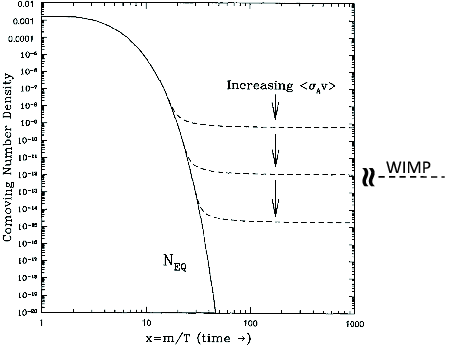
\includegraphics[width=0.7\textwidth]{IntroFigures/freezeout.png}
\caption{Comoving number density for WIMPs as a function of $\frac{M_{\chi}}{T}$.\label{fig:freezeout}}
\end{figure}

Now this annihilation rate can also be obtained from a particle
physics prospective by using a weak scale interaction strength. The
annihilation rate in this case is given by the following expression
(Fermi's golden rule):
\begin{equation}
\label{eq:FERMIGL}
\begin{aligned}
       &
\Gamma = \langle \sigma_{A}v\rangle = \frac{2\pi}{\hbar}|\mathcal{M}|^{2}\rho(E)
\qquad \text{with} \qquad \rho_{E} = \frac{4\pi}{\left(2\pi\hbar c\right)^{3}}E^{2},\\
\end{aligned}
\end{equation}
where $\mathcal{M}$ is the matrix element for the annihilation channel,
and $\rho(E)$ is the density of states, where we have assumed
relativistic particles in the final state. When the WIMPs are not
relativistic the final state particle obtain an energy ($E$) that is
equal to the mass of the WIMP. Now, assuming the simplest possible
annihilation channel where the matrix element squared
($\mathcal{M}|^{2}$) is just given by Fermi's constant squared
($G^{2}_{\mathrm{F}}$) we can compute the annihilation rate:
\begin{equation}
\label{eq:FERMIGL}
\begin{aligned}
      \langle \sigma_{A}v\rangle &
= \frac{1}{\pi}\frac{1}{\left(\hbar
    c\right)^{3}}G^{2}_{\mathrm{F}} M^{2}_{\chi}c^{4}\\
&
 = \frac{1}{\pi}\frac{\left(\hbar
    c\right)^{3}}{\hbar}(1.66\times 10^{-5}(\GeV)^{-2})^{2}
M^{2}_{\chi} (GeV)^{2}\\
 \langle \sigma_{A}v\rangle&\sim \frac{\left(\hbar
    c\right)^{3}}{\hbar} 10^{-10}(\GeV)^{-2}
M^{2}_{\chi}\\
\langle \sigma_{A}v\rangle&\sim  10^{-27} M_{\chi}\unit{cm}^{3}\unit{s}^{-1}
M^{2}_{\chi},\\
\end{aligned}
\end{equation}

where $M_{\chi}$ is in units of \GeV. Now we can readily see that a
WIMP mass at the weak scale (1\GeV-1\TeV) gives the correct order of
magnitude for the WIMP annihilation. The fact that WIMPS with a weak
scale interaction strength produces the necessary annihilation rate for a cold dark
matter relic obtained in Equation~\ref{eq:RELICDENSITY} -- purely from
astrophysical considerations -- is what some literature has named the
\textit{WIMP miracle}. 
\section{Searches for WIMP Dark Matter}
Three different type of experiments to search for WIMP dark matter are currently
underway. These searches are named, direct detection experiments,
indirect detection experiments, and particle collider
experiments. Figure~\ref{fig:dmDetection} shows a Feynman diagrams
with the possible ways in which WIMP DM can be detected, the dashed
blob represents the interaction of dark matter with the SM (quarks in
this case).

\begin{figure}
 \centering
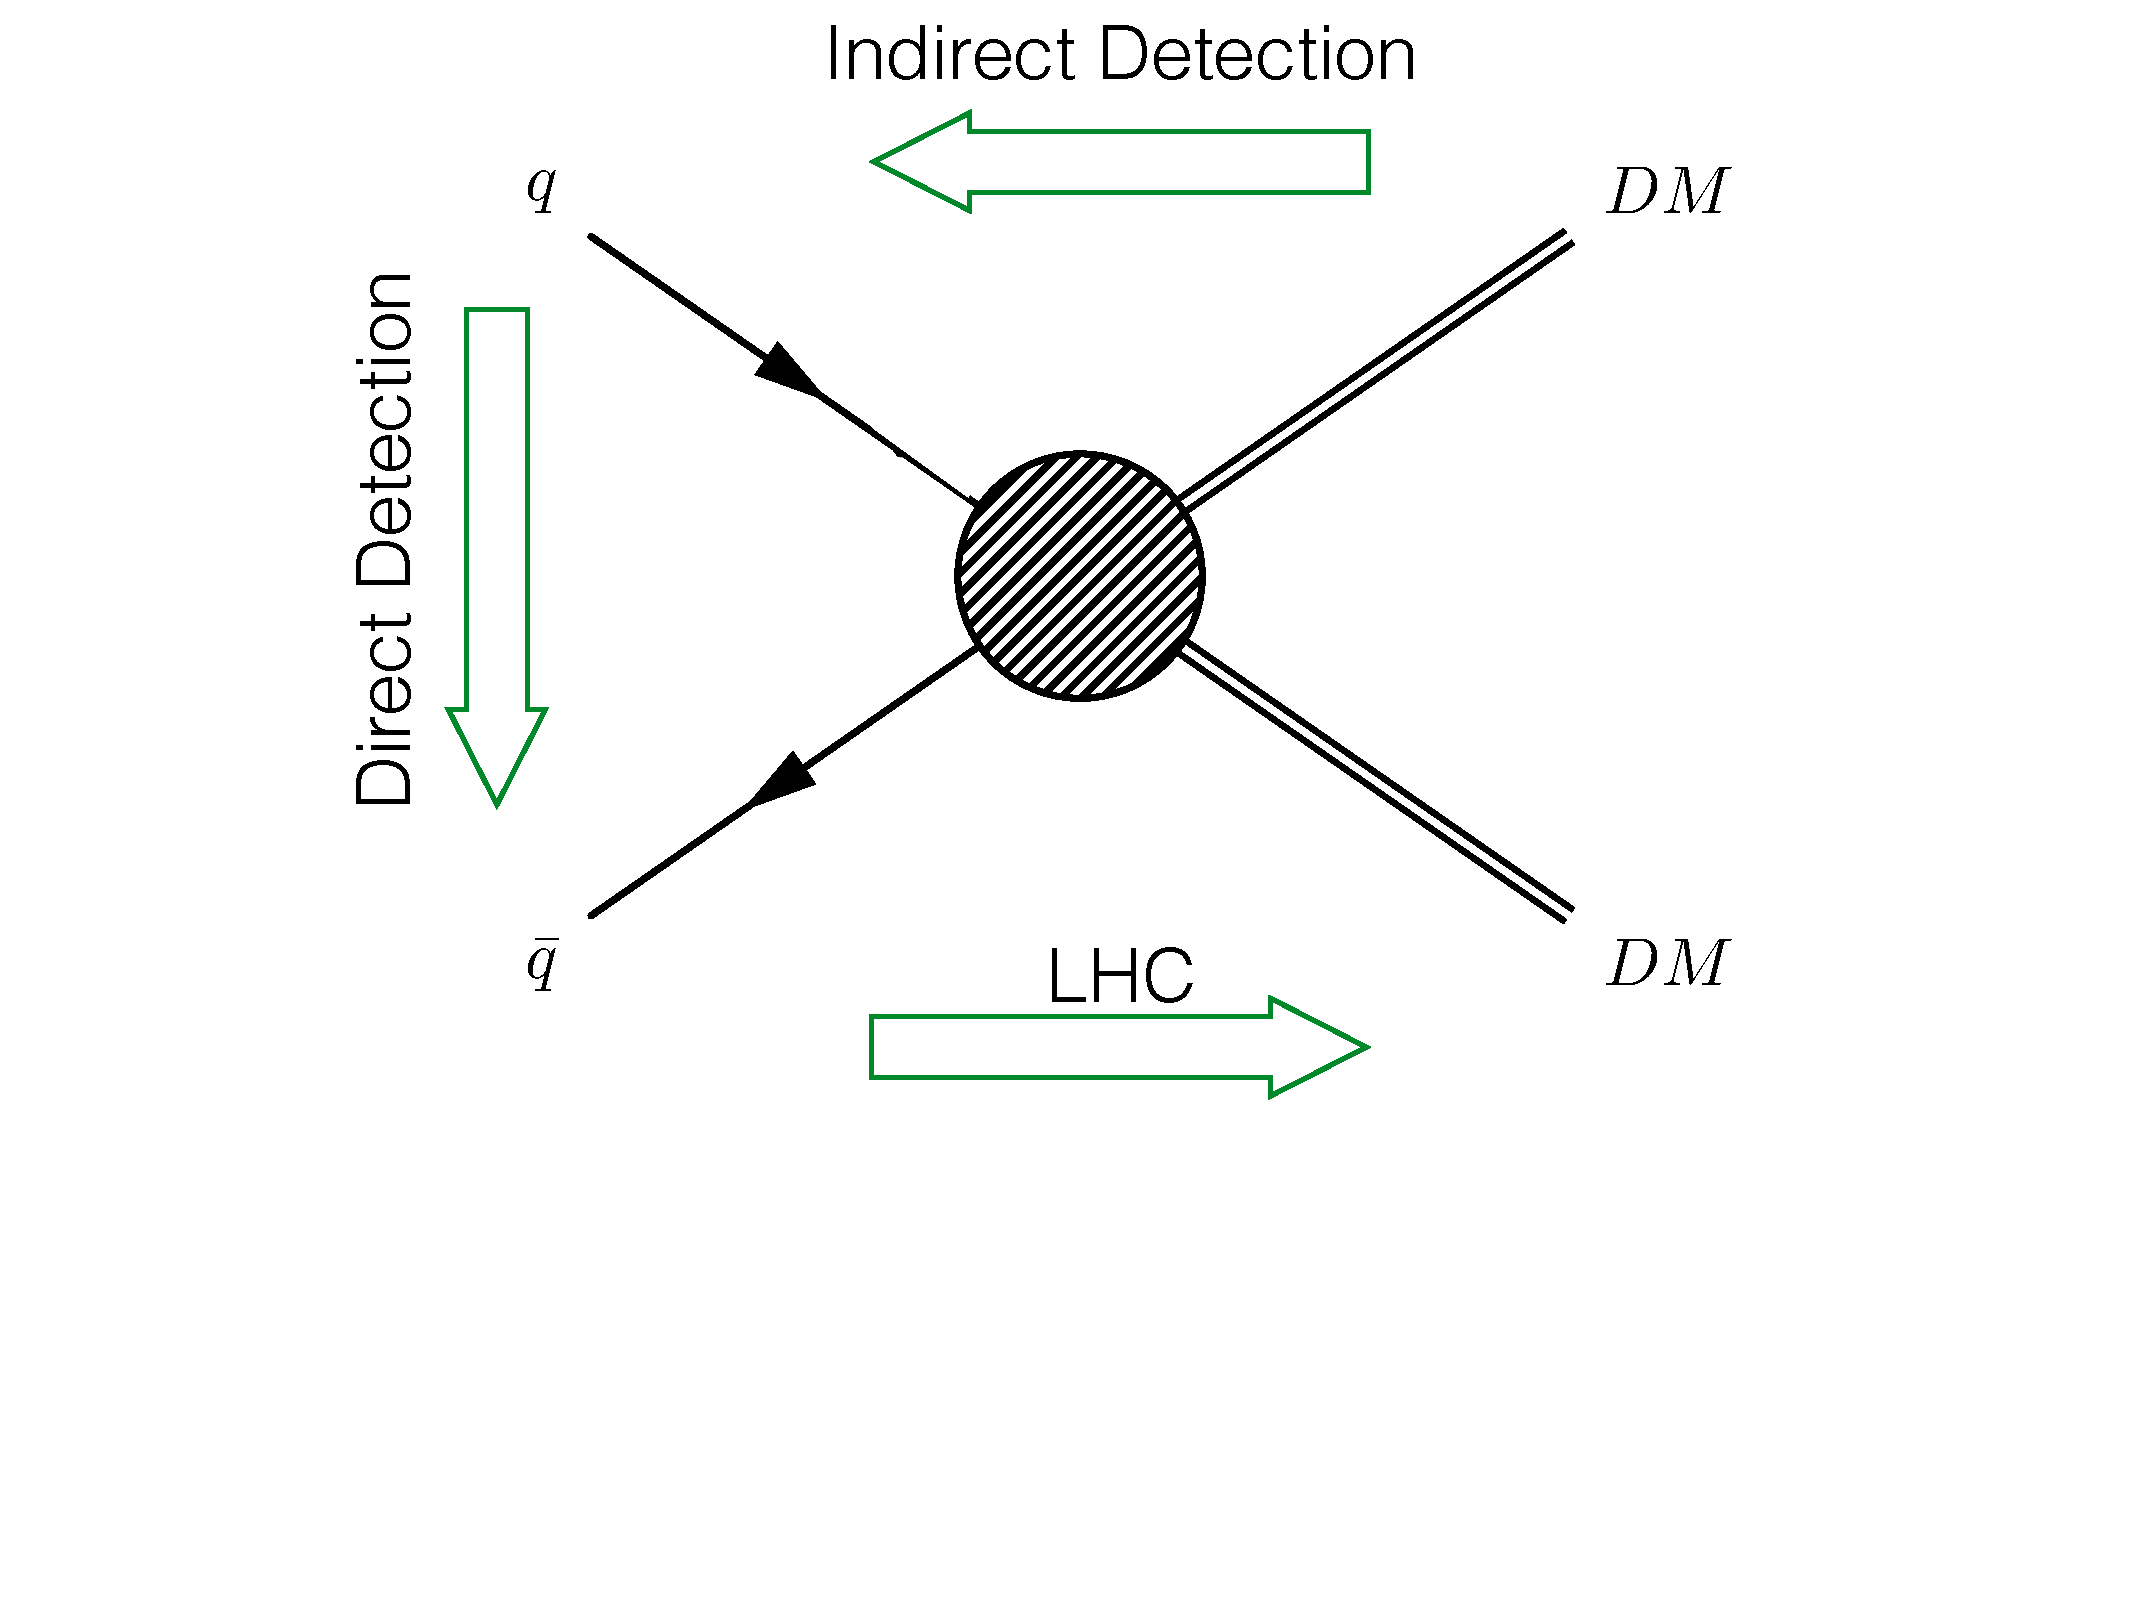
\includegraphics[width=0.6\textwidth]{IntroFigures/DiagramDMdetection.pdf}
\caption{Feynman diagram including the possible manner in which DM can
  be experimentally detected. The green arrows indicate the
  orientation in which the diagram should be read to produce a
  particular detectable signal.\label{fig:dmDetection}}
\end{figure}

\subsection{Direct detection}
Direct detection experiments are based on WIMP-nucleus scattering
which in turn depend on the WIMP-quark cross-section. Assuming a
standard WIMP scenario the WIMP-nucleus cross section is of the order
of $10^{-36}$\unit{cm}$^{2}$, which yields a detectable rate of
interactions of about 1 event per kilogram per day. This requires
large mass detector and large exposure times in order to increase the
possibilities to detect WIMPs. Another consideration in direct
detection experiments is the amount of energy transferred to the
nucleus by the WIMP and the ability to record that energy. In an
elastic collision the energy transfer to the nucleus (recoil energy)
is

\begin{equation}
\label{eq:recoilE}
E_{\mathrm{recoil}} = \frac{2\frac{M_{\mathrm{N}}}{M_{\mathrm{DM}}}}{\left(1+\frac{M_{\mathrm{N}}}{M_{\mathrm{DM}}}\right)^{2}}E_{\mathrm{DM}},
\end{equation}

where $E_{\mathrm{recoil}}$ is the recoil energy, $M_{\mathrm{N}}$ is
the nucleus mass, $M_{\mathrm{DM}}$ is the DM mass (assumed to be
around 100\GeV), and $E_{\mathrm{DM}}$ is the DM kinetic energy
(assuming a velocity of about 270\unit{km/s} yield a kinetic energy of
about 50\keV). Assuming an nucleus with an atomic weight of about
72-131 (Germanium and Xenon, respectively), the recoil energy is about
25 keV (note that the maximum kinetic energy is in fact just twice the
DM kinetic energy). The experimental techniques used include detection
of thermal/phonons fluctuations, ionization detectors, and scintillator
detectors. No evidence of a DM detection has been announced and
the current DM-nucleon cross-section limits are presented in
Figure~\ref{fig:dmLimits}. 
\begin{figure}
 \centering
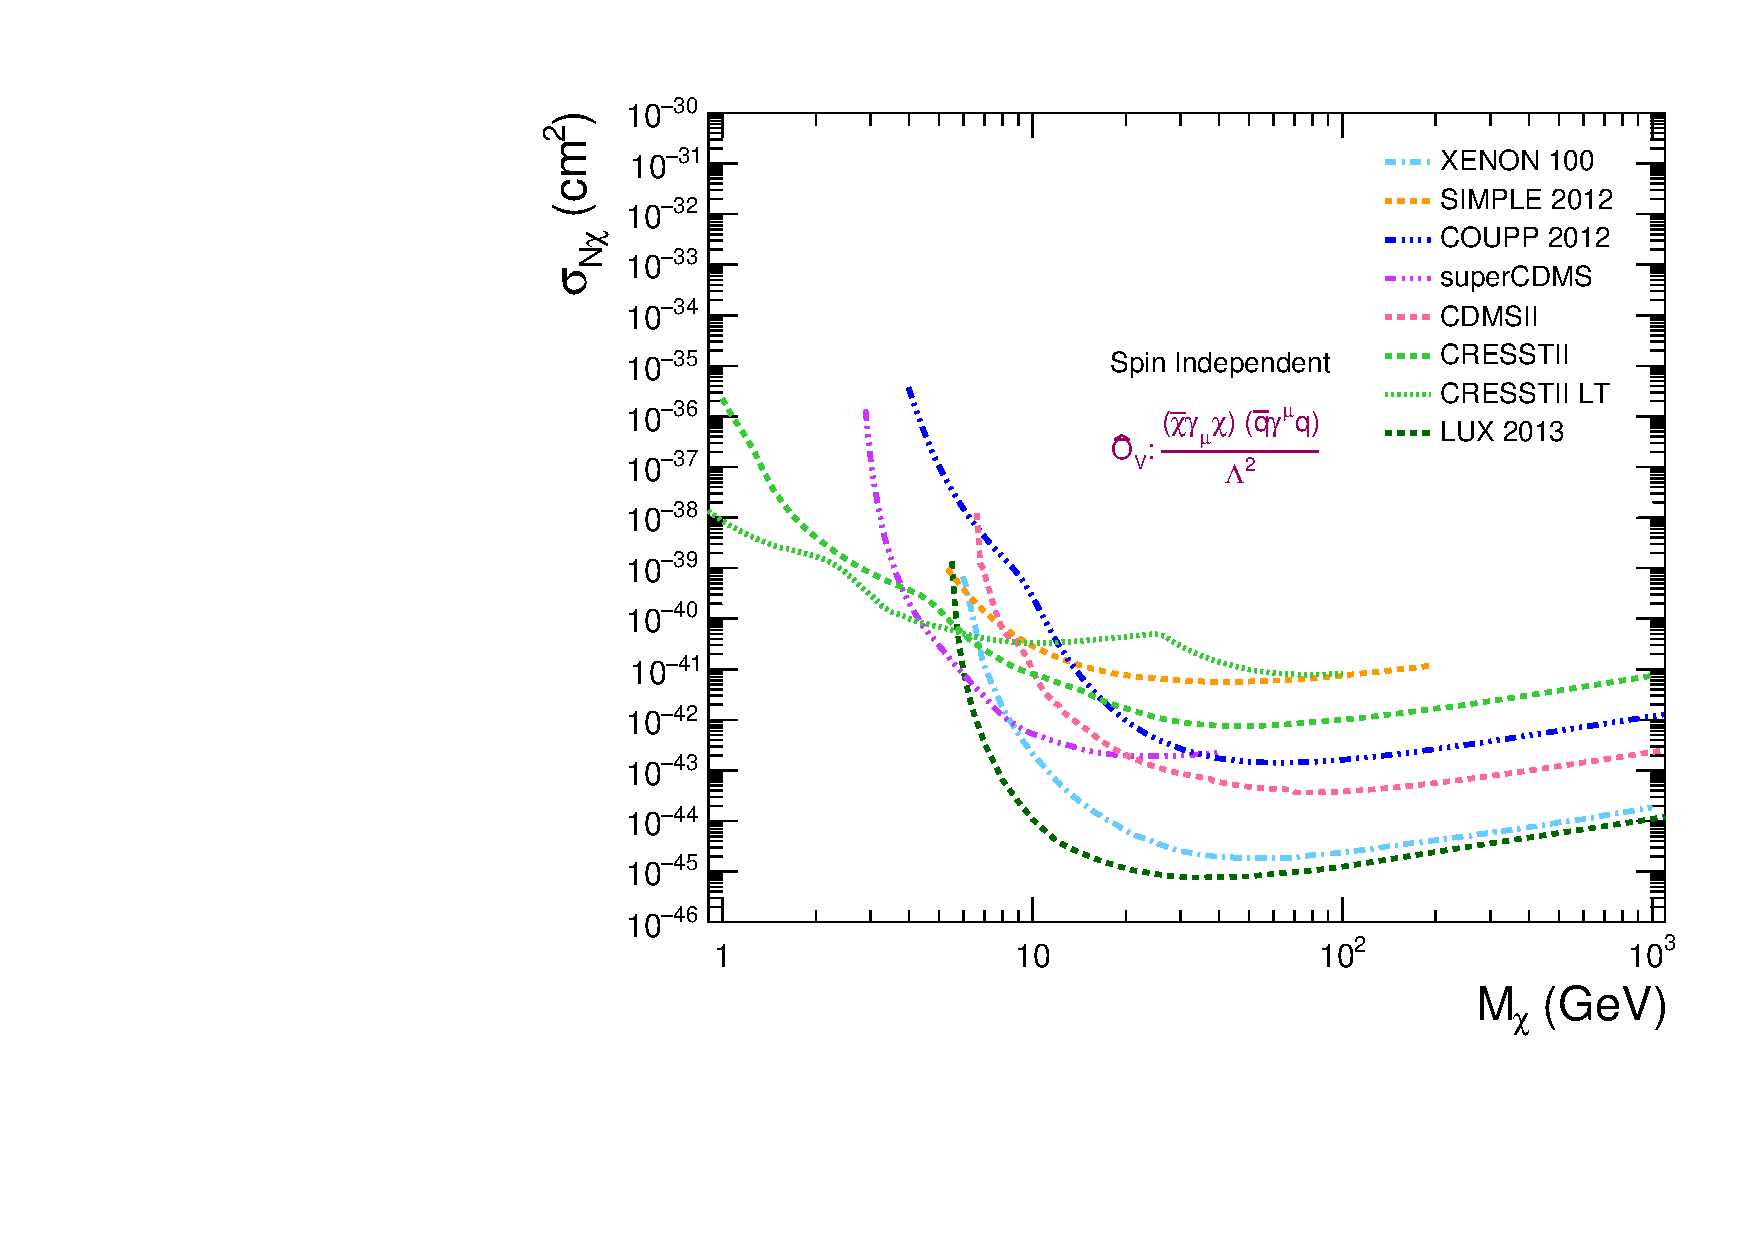
\includegraphics[width=0.6\textwidth]{IntroFigures/SI_DM.pdf}
\caption{Spin-independet DM-nucleon cross section ($\sigma_{N\chi}$) exclusion limits
  as a function of the DM candidate mass ($M_{\chi}$) from direct detection experiments.\label{fig:dmLimits}}
\end{figure}
\subsection{Indirect detection}
Assuming WIMP dark matter, the same mechanism by which the observed
relic density was obtained at the early stages of the universe,
i.e. WIMP-WIMP annihilation, should still be taking place in regions
where there are large amounts of dark matter. The annihilation
rate is proportional to the  WIMP density squared
($\Gamma_{\chi\chi\rightarrow X} \propto n^{2}_{\chi}$, where $\chi$
represents the WIMP), therefore the detection is increased when
looking at regions of high DM density such as the Earth, the sun, and
the galactic center. This annihilation signature is looked for in
different channels that ultimately will produce excess of gamma-rays,
neutrinos, or anti-particles -- particularly positrons. These
astrophysical searches are classified as \textit{indirect
  detection}~\cite{IND1,IND2}, since WIMPs are not directly detected. 

Gamma-rays could be produce by the $\chi\chi\rightarrow q\bar{q}$
reaction (specially in the galactic center), subsequently the quarks will hadronize and produce photons
that can be detected by a particle detector; the limitation of this
mode is that only as a continuum excess. Another reactions that could
produce an enhancement of gamma-rays are $\chi\chi\rightarrow
\gamma\gamma$ and $\chi\chi\rightarrow
\gamma Z$, where the excess will be observed by a line in the
gamma-ray spectrum. The EGRET collaboration reported an excess of
events in their gamma-ray spectrum in 1998\cite{EGRETT}, indicating a
standard WIMP scenario. The EGRET excess remains controversial due to
the null observation in the antiproton flux. The Fermi Gamma-ray Space
Telescope (Fermi-LAT) launched in 2008~\cite{FERMILAT} has also observed some
excesses coming from the galactic center~\cite{FermiExcess}, though encouraging results,
the community await for more data to be collected to elucidate these
hints of DM detection. Figure~\ref{fig:FERMI} shown the gamma-ray map
collected by FERMI-LAT.

\begin{figure}
 \centering
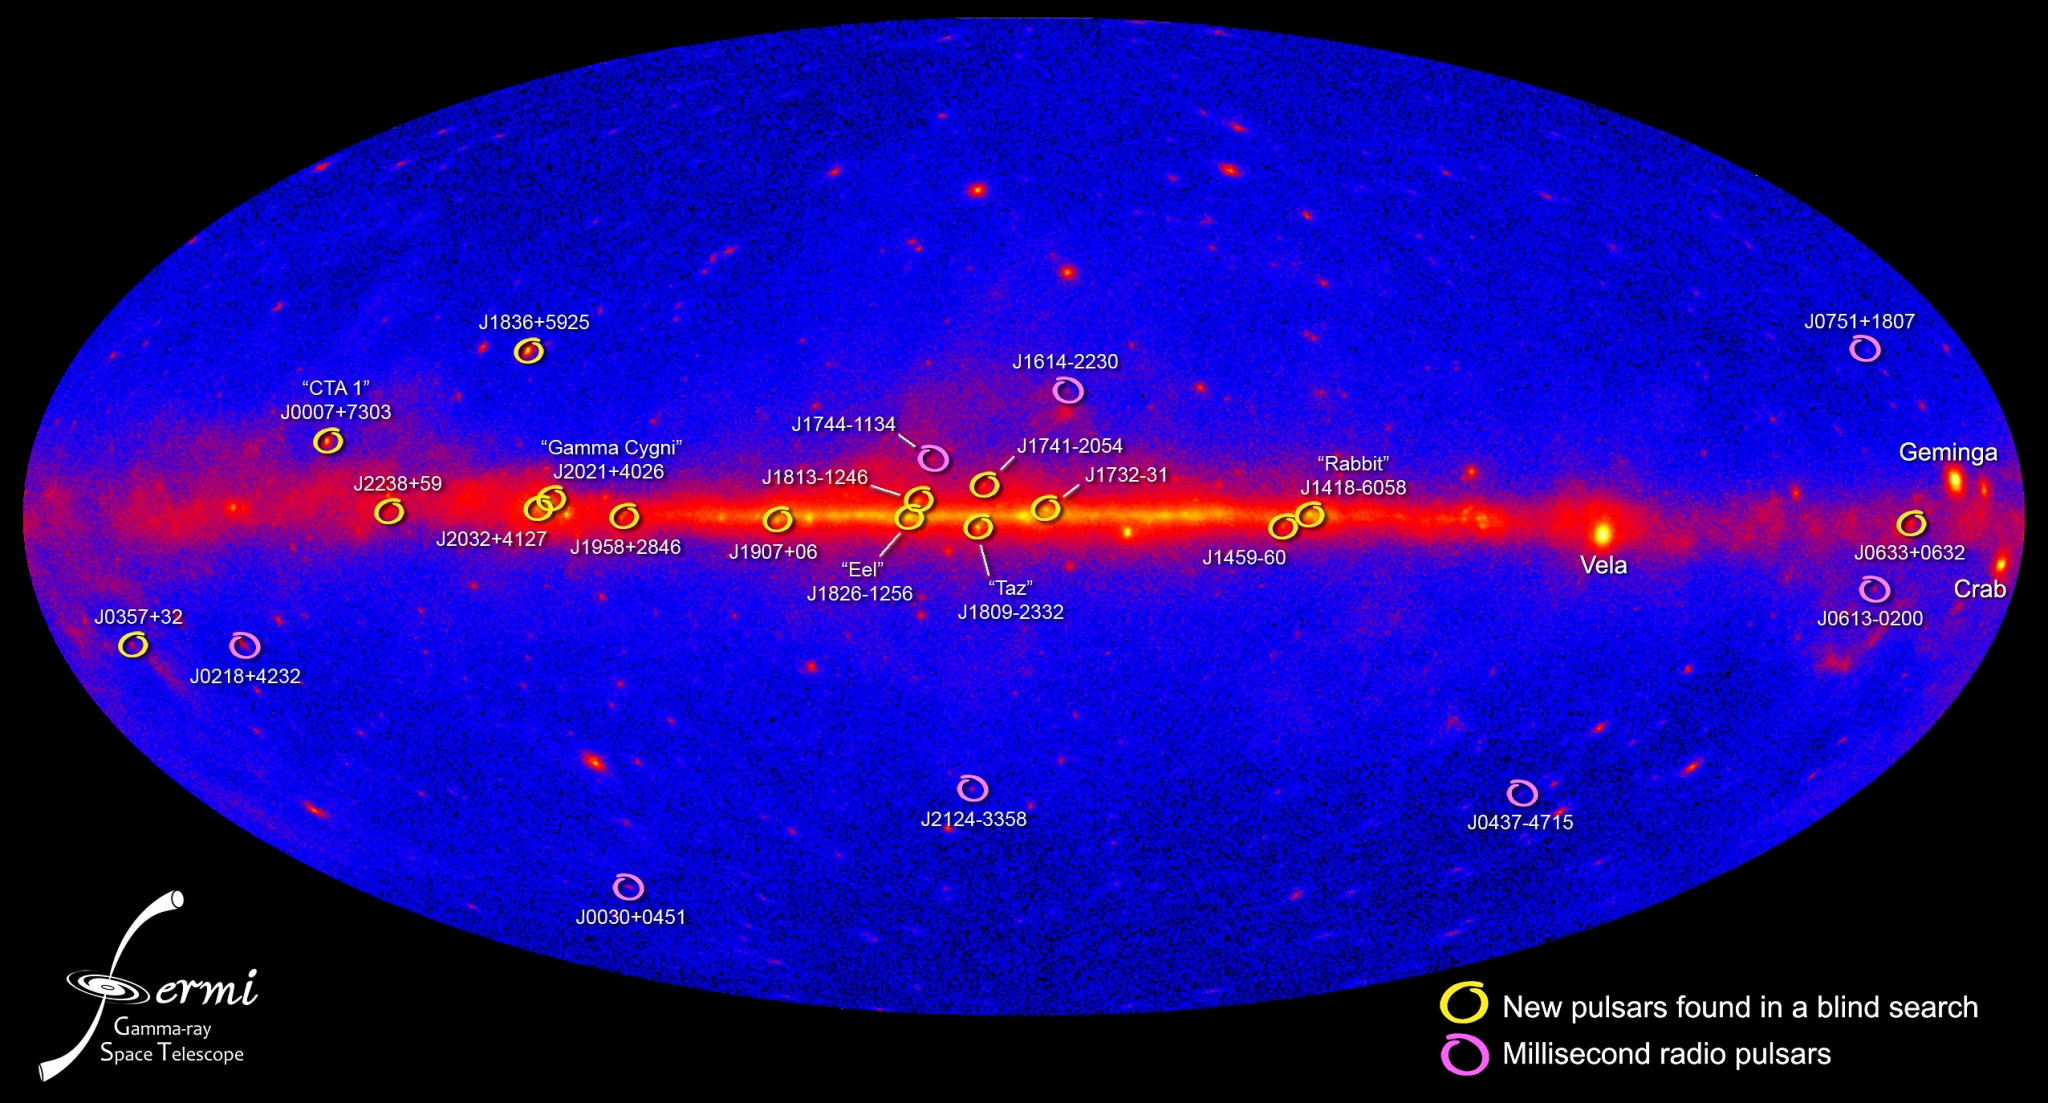
\includegraphics[width=0.9\textwidth]{IntroFigures/Fermi_Map.jpg}
\caption{The gamma-ray sky as mapped by the FERMI-LAT satellite.\label{fig:FERMI}}
\end{figure}

Excess of neutrino flux can also indicate the presence if WIMP dark
matter. The sun is  good place to look for neutrino flux excesses
since the solid angle for annihilation is greatly increased with
respect to that of the galactic center. Processes such as
$\chi\chi\rightarrow t\bar{t}, b\bar{t}, c\bar{c}, ZZ, W^{+}W^{-},$ and
$\tau^{+}\tau^{-}$ will lead to neutrino final states. Detectors can
be located in Earth since  neutrinos interact very weakly with
matter. Large detector such as IceCube, Super-Kamiokande, among other, are already in place trying to detect DM by
observing neutrino flux excesses.

Since anti-matter is rare in our universe, search for excesses of
anti-particles is an attractive way to observed WIMP annihilation --
particularly those producing positrons and antiprotons. Again,
positrons can be produced directly or as decay product of other SM
particles, while antiprotons via quark hadronization. The PAMELA
satellite\cite{PAMELA} has observed an excess of events with positron energies
between 1.5-100\GeV\cite{PAMELAEXCESS}. As
in the gamma-ray excesses, larger data samples are needed to confirm or
disprove the current observations, such data sets will be provided by
FERMI-LAT.

\subsection{Searches for dark matter production at the LHC}
Dark matter could be produced at the LHC as a decay product of heavier
states in the context of SUSY, this will result in a signature with a
variety of SM particles in the final state along with missing
transverse-momentum due to the weakly interacting nature of the DM
candidate -- the lightest neutralino.  A different approach to search
for dark matter in particle colliders which involves different
couplings between the the relevant SM particles at the LHC and the DM
candidate has been adopted by the ATLAS and CMS collaborations. These
interactions involve different non-renormalizable effective operators
-- in the context of quantum field theory -- where the mediating
force carried field is assumed to be above the LHC energies and
therefore \textit{integrated out}. A list of the possible effective
operators in shown in Table~\ref{tab:EFT}. The most popular
operator studied in the 7 and 8\TeV run of the LHC where the
\textit{vector} and \textit{axial-vector} operators, which can be
translated to spin-independent and spin-dependent DM-nucleon cross
section and be compared to the results obtained by direct detection
experiments. This comparison is the result of a series of assumptions
in both experiments and therefore they should be interpreted with
caution. These event topologies will not be recorded in the particle
detectors since they produce two DM candidates in the
final state that will completely scape detection. Therefore another
high-$p_{\mathrm{T}}$ particle needs to be produce in order to
activate the trigger systems deployed in modern particle
detectors. This extra requirement is satisfied by the production of
initial-state-radiation off the quarks (see left panel of
Figure~\ref{fig:DMdiamgrams}). Such events topologies became to be
know as \textit{mono-X}, where X denotes the high-$p_{\mathrm{T}}$
object that could be a jet, photon, lepton, Z/W bosons, or a Higgs
boson, among others. Figure~\ref{fig:CMSlimits} shows the
spin-independent results from the mono-jet and mono-photon analyses
released by the CMS
collaboration~\cite{Aad:2011xw,Chatrchyan:2012me,Khachatryan:2014rwa,Aad:2014tda}. The
effective field theory approach to obtain the operators in
Table~\ref{tab:EFT} turned out to be violated in a portion
of the events recored at the LHC and therefore their bounds are not
completely accurate~\cite{Riotto1,Riotto2,Riotto3}. Attempts to solve this issue are now in
place by including the mediator particle and the coupling strength to
be parameters of the model~\cite{DMFORUM}. Chapter~\ref{DMatLHC} presents a
search for particle DM in events with two or more jets, providing the
LHC searches with a inclusive analysis approach that is at the same
time complementary to the existing mono-jet searches by ATLAS and
CMS. This search also quantifies the amount fraction of events that
violate the EFT assumption.

\begin{table}[htb]
\centering
\large
\begin{tabular}{cccc}
  \hline
  \hline
  Name &  Initial state &  Type & Operator\\
  \hline                                                        
  D1 & $q\bar{q}$ &  scalar & $\frac{m_{q}}{M^{3}_{*}}\bar{\chi}\chi\bar{q}q$\\
  D5 & $q\bar{q}$ & vector & $\frac{1}{M^{2}_{*}}\bar{\chi}\gamma_{\mu}\chi\bar{q}\gamma^{\mu} q$\\
  D8 & $q\bar{q}$ &  axial-vector & $\frac{1}{M^{2}_{*}}\bar{\chi}\gamma_{\mu}\gamma^{5}\chi\bar{q}\gamma^{\mu}\gamma^{5} q$\\
  D9 & $q\bar{q}$ &  tensor & $\frac{1}{M^{2}_{*}}\bar{\chi}\sigma_{\mu\nu}\chi\bar{q}\sigma^{\mu\nu} q$\\
  D11 & $gg$ &  scalar & $\frac{1}{M^{3}_{*}}\bar{\chi}\chi\alpha_{s}(G^{s}_{\mu\nu})^2$\\
  \hline
  \hline
\end{tabular}
  \caption{\label{tab:EFT}A selection of the possible effective operators for DM production at
    the LHC~\cite{EFTColliders}. $M_{*}$ is the cutoff scale of
    the effective operator (sometimes this quantity is also
    represented by $\Lambda$).}
\end{table}

\begin{figure}
 \centering
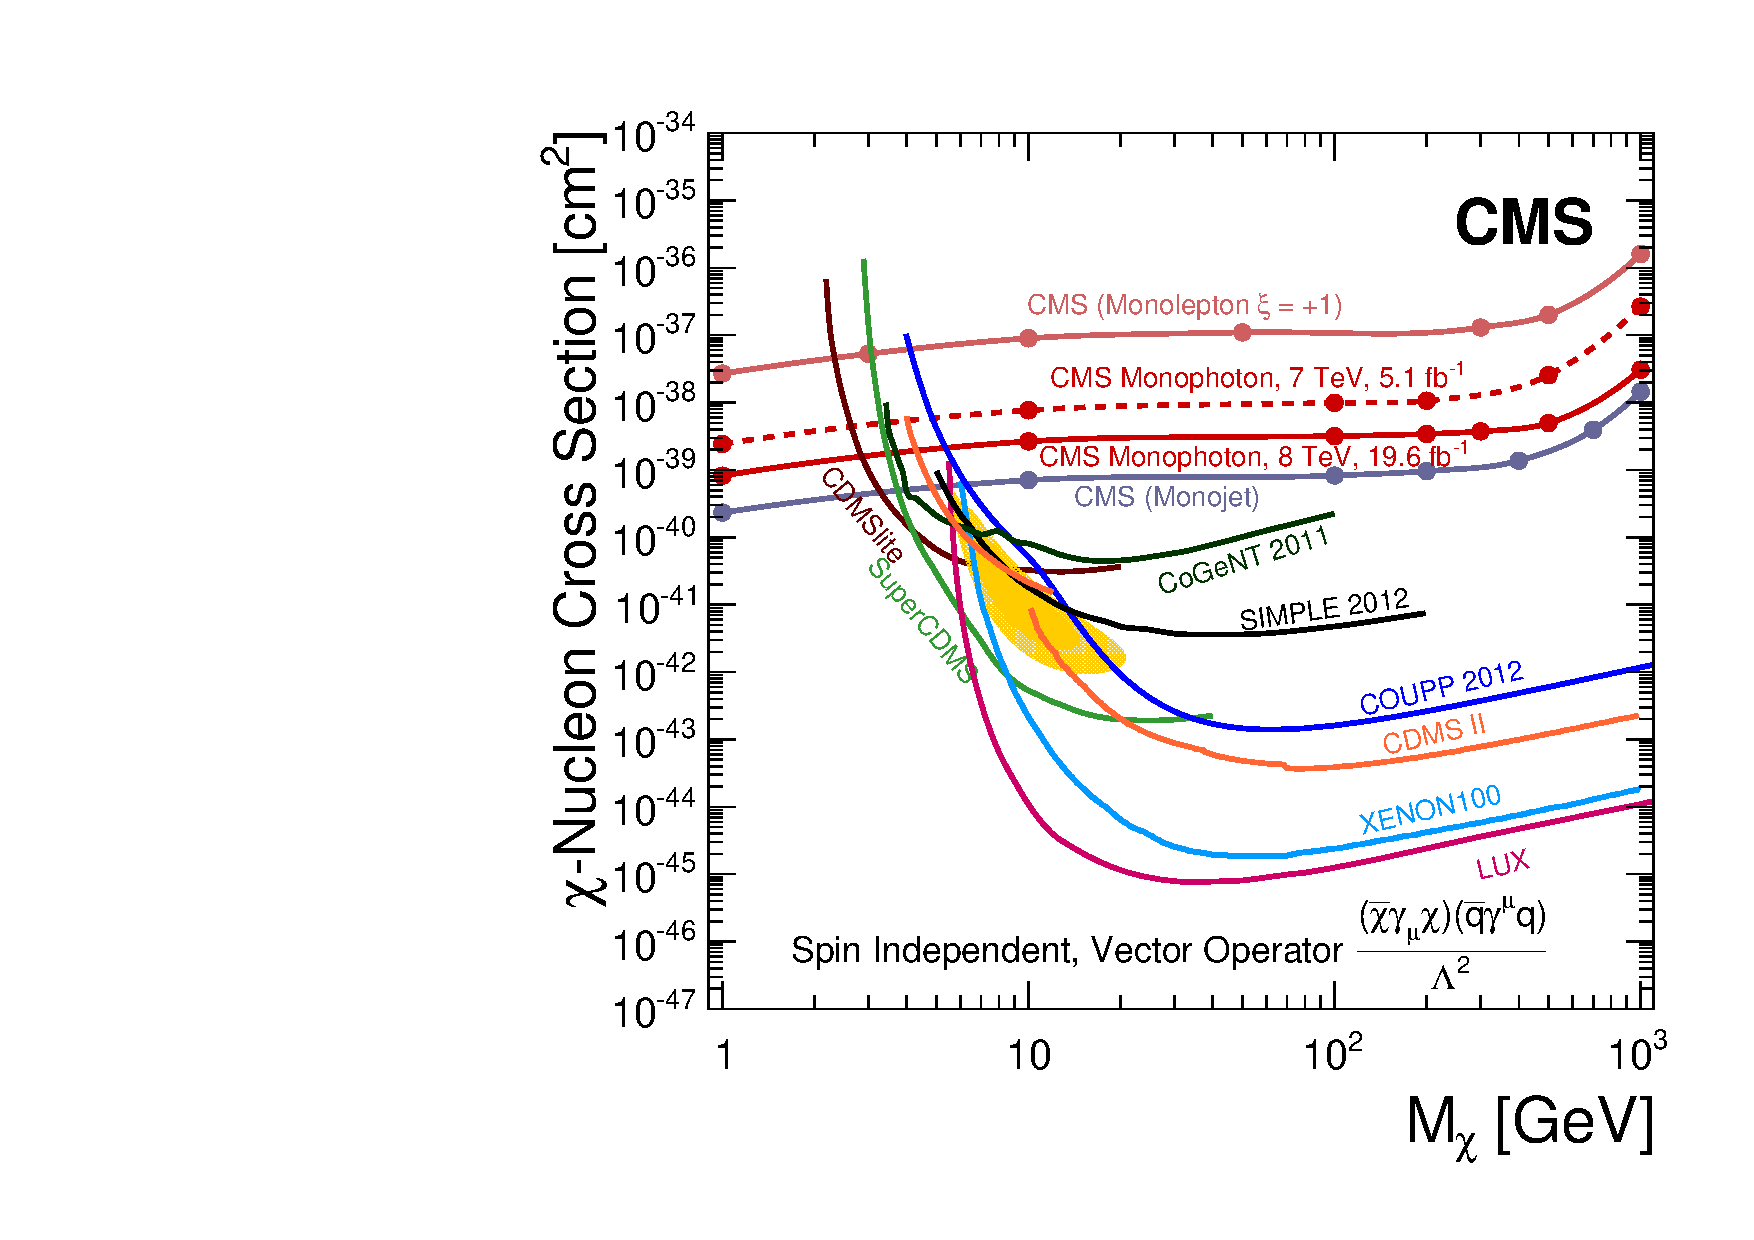
\includegraphics[width=0.7\textwidth]{IntroFigures/dm_limit.pdf}
\caption{The DM-nucleon cross section 90\% CL. bounds published by
  the CMS mono-jet
  and mono-photon searches.\label{fig:CMSlimits}}
\end{figure}